\documentclass[12pt,openany]{book}

\usepackage[T1]{fontenc}
\usepackage[utf8]{inputenc}
\usepackage{amsmath,amsthm,mathtools}
\usepackage{centernot}
\usepackage{newtxtext,newtxmath}
\usepackage{microtype}
\usepackage[a4paper,inner=30mm,outer=24mm,top=27mm,bottom=28mm,headheight=16pt]{geometry}
\usepackage{graphicx}
\usepackage{xcolor}
\usepackage{bm}
\usepackage{booktabs,longtable,array,tabularx}
\usepackage{enumitem}
\usepackage{tikz}
\usetikzlibrary{arrows.meta,positioning,calc,fit,backgrounds,decorations.pathmorphing,shapes.geometric}
\usepackage[most]{tcolorbox}
\usepackage{fancyhdr}
\usepackage{titlesec}
\usepackage{caption}
\usepackage{subcaption}
\usepackage{epigraph}
\usepackage{setspace}
\usepackage{csquotes}
\usepackage{hyperref}
\usepackage[nameinlink,noabbrev]{cleveref}

\definecolor{Midnight}{HTML}{07111F}
\definecolor{DeepBlue}{HTML}{173B67}
\definecolor{IceBlue}{HTML}{DCEEFF}
\definecolor{Teal}{HTML}{2B8C88}
\definecolor{Violet}{HTML}{7051A6}
\definecolor{Gold}{HTML}{B78A38}
\definecolor{Rose}{HTML}{A64F6A}
\definecolor{Slate}{HTML}{485666}
\definecolor{SoftGray}{HTML}{F1F3F5}

\hypersetup{
  colorlinks=true,
  linkcolor=DeepBlue,
  citecolor=Teal,
  urlcolor=Violet,
  pdftitle={The Weave Never Ends},
  pdfauthor={Jesus Jose Vilela Jato},
  pdfsubject={Hardness, Infinite Holonomy, and the Recursive Geometry of Faithful Return},
  pdfkeywords={hardness, holonomy, profunctor, protensor, fiber bundle, braid, hypercomplex, cosmocomplexity}
}

\pagestyle{fancy}
\fancyhf{}
\fancyhead[LE]{\small\scshape The Weave Never Ends}
\fancyhead[RO]{\small\scshape\nouppercase{\leftmark}}
\fancyfoot[C]{\thepage}
\renewcommand{\headrulewidth}{0.4pt}

\titleformat{\chapter}[display]
  {\normalfont\huge\bfseries\color{Midnight}}
  {\filleft\Large\color{Gold}\chaptername\ \thechapter}
  {1ex}
  {\titlerule[0.8pt]\vspace{1.2ex}\filright}
  [\vspace{1ex}\titlerule]
\titleformat{\section}{\Large\bfseries\color{DeepBlue}}{\thesection}{0.7em}{}
\titleformat{\subsection}{\large\bfseries\color{Teal}}{\thesubsection}{0.6em}{}

\newtheorem{definition}{Definition}[chapter]
\newtheorem{principle}[definition]{Principle}
\newtheorem{proposition}[definition]{Proposition}
\newtheorem{conjecture}[definition]{Conjecture}
\newtheorem{theoremseed}[definition]{Theorem-seed}
\newtheorem{warning}[definition]{Boundary warning}
\newtheorem{openproblem}[definition]{Open problem}
\theoremstyle{remark}
\newtheorem{remark}[definition]{Remark}
\newtheorem{example}[definition]{Example}

\newtcolorbox{invariantbox}[1][]{
  enhanced,
  colback=IceBlue!45,
  colframe=DeepBlue,
  boxrule=0.8pt,
  arc=2mm,
  title={#1},
  fonttitle=\bfseries,
  left=3mm,right=3mm,top=2mm,bottom=2mm
}
\newtcolorbox{remainderbox}[1][]{
  enhanced,
  colback=Rose!6,
  colframe=Rose,
  boxrule=0.8pt,
  arc=2mm,
  title={#1},
  fonttitle=\bfseries,
  left=3mm,right=3mm,top=2mm,bottom=2mm
}
\newtcolorbox{claimbox}[1][]{
  enhanced,
  colback=Gold!8,
  colframe=Gold!80!black,
  boxrule=0.8pt,
  arc=2mm,
  title={#1},
  fonttitle=\bfseries,
  left=3mm,right=3mm,top=2mm,bottom=2mm
}

\DeclareMathOperator{\Hol}{Hol}
\DeclareMathOperator{\Obs}{Obs}
\DeclareMathOperator{\Ret}{Ret}
\DeclareMathOperator{\Rec}{Rec}
\DeclareMathOperator{\Rep}{Representable}
\DeclareMathOperator{\Rel}{Rel}
\DeclareMathOperator{\Id}{Id}
\DeclareMathOperator{\im}{Im}
\DeclareMathOperator{\cofib}{cofib}
\DeclareMathOperator{\argmax}{arg\,max}
\DeclareMathOperator{\Compare}{Compare}
\DeclareMathOperator{\Transport}{Transport}
\DeclareMathOperator{\Weave}{Weave}
\DeclareMathOperator{\Unweave}{Unweave}
\newcommand{\Nfabric}{\mathcal N}
\newcommand{\Remainder}{[R]}
\newcommand{\WTheta}{\mathfrak W_{\Theta}}
\newcommand{\UTheta}{\mathfrak U_{\Theta}}
\newcommand{\Hard}{\mathcal H}
\newcommand{\Fabric}{\mathcal F}
\newcommand{\Cosmos}{\mathfrak X}
\newcommand{\Protensor}{\mathbb P}
\newcommand{\DiamondHol}{\Omega_{\diamond}}
\newcommand{\wideZ}{\widehat{\mathbb Z}}
\newcommand{\typedtuple}[1]{\left\langle #1 \right\rangle}

\setstretch{1.08}
\setlist[itemize]{leftmargin=2em,itemsep=0.25em,topsep=0.4em}
\setlist[enumerate]{leftmargin=2em,itemsep=0.3em,topsep=0.4em}

\begin{document}

\begin{titlepage}
\pagecolor{Midnight}
\color{white}
\centering
\vspace*{1.1cm}
{\Huge\bfseries THE WEAVE NEVER ENDS\par}
\vspace{0.4cm}
{\Large Hardness, Infinite Holonomy, and the Recursive Geometry of Faithful Return\par}
\vspace{0.35cm}
{\large The Definitive LaTeX Edition\par}
\vspace{0.9cm}
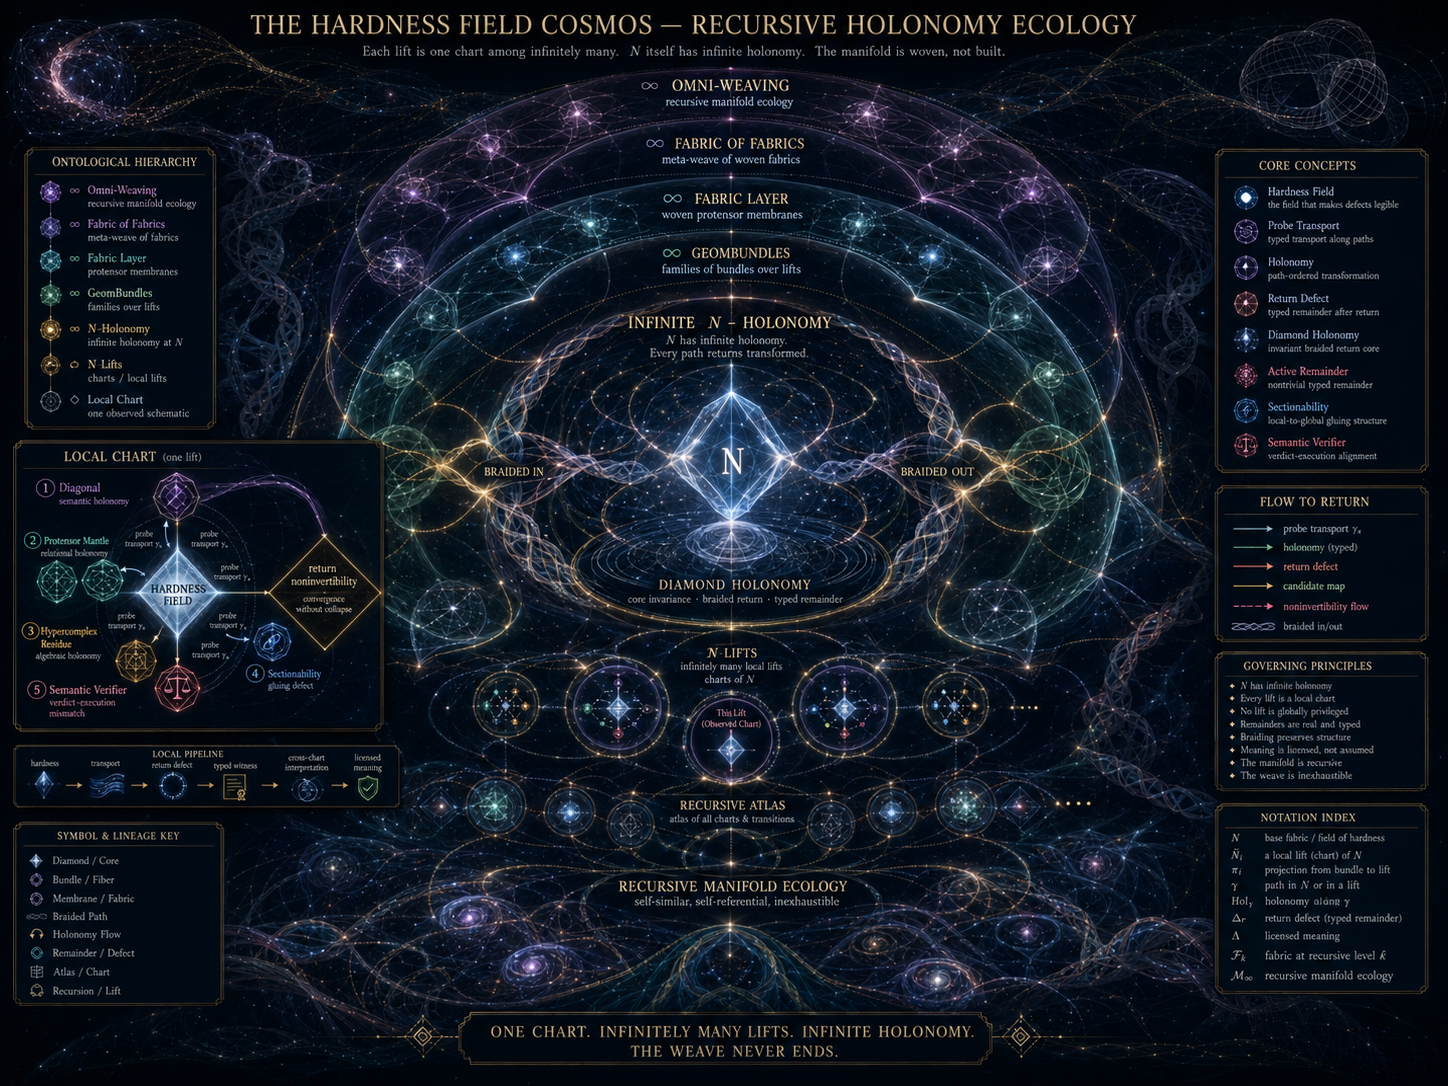
\includegraphics[width=0.88\textwidth]{assets/recursive_holonomy_cosmos.png}
\vfill
{\Large Jesus Jose Vilela Jato\par}
\vspace{0.2cm}
{\normalsize Research programme manuscript - Madrid - July 2026 - Revision r2\par}
\vspace{0.6cm}
{\small A moving atlas of omni-weaving, un-generation, braided fabrics, split-signature cables, and cosmocomplex emergence.\par}
\end{titlepage}
\nopagecolor
\color{black}

\pagenumbering{roman}
\chapter*{Epigraph}
\addcontentsline{toc}{chapter}{Epigraph}
\begin{epigraphs}
\qitem{The question is not whether a result returns. The question is whether the complete relation that made it true can return.}{Governing formulation}
\qitem{One chart. Infinitely many lifts. Infinite holonomy. The weave never ends.}{Recursive holonomy doctrine}
\end{epigraphs}

\chapter*{Abstract}
\addcontentsline{toc}{chapter}{Abstract}
This thesis develops a moving geometric programme for the study of hardness. Hardness is not treated as a scalar quantity, a frozen property of an isolated object, or a synonym for computational cost. It is treated as the field that makes failures of faithful return legible when an object is transported through representation, self-reference, algebraic transformation, relational composition, observation, and verification.

A probe entering this field may return to the same visible endpoint while failing to return with the relation that made the endpoint meaningful. Witnesses may disappear; provenance may be severed; route order may be compressed; parenthesization may be lost; locally compatible sections may fail to glue; a verdict may survive while the execution relation supporting it does not. These path-dependent return defects are called holonomies. Hardness is not identified with any one holonomy. Hardness is the moving field interrogated by a family of heterogeneous probes; holonomy is the typed remainder brought back by each probe.

The local engine of the programme is a paired weaving geometry
\[
\WTheta \dashv \UTheta,
\]
where the omni-weaver generates, braids, glues, and hybridizes relational structure, while the un-gen-weaver interrogates the generated object for the fibers, mediators, witnesses, provenance, braid history, association tree, and unresolved remainder from which it arose. Their relation is targeted as an adjunction rather than a naive inverse; the existence of that adjunction on explicitly constructed categories is itself a registered theorem-seed, and only the unit--counit interface is treated as defined. Hardness becomes visible where generation succeeds but licensed un-generation cannot reconstruct the complete generating ecology.

The transport substrate combines a split-signature cable $\mathbb R^{2,2}$, a profinite phase tower $\wideZ$, hypercomplex transport, protensorial membranes, and an active remainder. These carriers preserve, respectively, productive and destructive coupling directions, compatible finite return residues, noncommutative and potentially nonassociative history, mediated relational composition, and what the current atlas cannot yet reconstruct. The resulting architecture refuses scalar certification: a scalar may probe a chart, but it cannot certify the woven relational object.

The thesis then lifts from fibers and bundles to fabrics, fabrics of fabrics, and recursively woven manifold ecologies. The base fabric $\Nfabric$ admits infinitely many local lifts, but the infinite holonomy of $\Nfabric$ is not exhausted by their enumeration. Each fabric may itself become a fiber of a higher fabric; each law of weaving may become an object requiring further weaving; each apparently global closure remains local while an active remainder survives.

The research target is a licensed diamond holonomy: independently typed return defects converge only after explicit witness-sensitive interpretation maps transport them into a shared invariant carrier. No convergence is accepted by metaphor, repeated labels, or constant codomain collapse. The programme therefore distinguishes defined structure, proved structural results, conditional semantic licensing, tested operational shadows, open conjectures, and unsafe identifications.

The governing thesis is:
\begin{invariantbox}[Central thesis]
Hardness becomes observable where generation succeeds, but no licensed, witness-preserving return equivalence can reconstruct the complete relation that made the generated object possible.
\end{invariantbox}

\chapter*{Reader's Orientation and Claim Discipline}
\addcontentsline{toc}{chapter}{Reader's Orientation and Claim Discipline}
This manuscript is deliberately ambitious in ontology and conservative in licensing. It should be read simultaneously in three registers.

\begin{enumerate}
\item \textbf{Geometric register.} Bundles, connections, holonomy, split signatures, hyperbolic motion, and moving frames provide the language of transport and non-return.
\item \textbf{Relational register.} Profunctorial and protensorial carriers retain mediators, witnesses, provenance, routes, and remainder through composition.
\item \textbf{Operational register.} Every higher construction is required to admit finite audit shadows, explicit comparison records, or formal interfaces before it may support stronger claims.
\end{enumerate}

The word \emph{protensor} is used as coined operational terminology for an enriched, witnessed, provenance-bearing, remainder-preserving profunctorial carrier. The thesis does not present it as universally established nomenclature. Likewise, references to coends, cofibers, higher adjunctions, and nonassociative transport are always conditioned on the existence of the structures required to define them. Where those structures are not yet formalized, the manuscript states an operational shadow rather than silently importing the completed theory.

The manuscript has no terminal claim that hardness has been solved, that the Halting Problem has been resolved, or that all return defects are instances of one already constructed invariant. Its definitive character lies elsewhere: it gives the most complete current atlas of the programme, states the type boundaries, preserves the active remainder, and converts the principal intuitions into theorem-seeds and falsifiable research obligations.

\tableofcontents
\listoffigures

\chapter*{Notation at a Glance}
\addcontentsline{toc}{chapter}{Notation at a Glance}
\begin{longtable}{>{\raggedright\arraybackslash}p{0.18\textwidth}>{\raggedright\arraybackslash}p{0.72\textwidth}}
\toprule
Symbol & Meaning \\
\midrule
\endhead
$\Hard$ & The moving hardness field. \\
$\Nfabric$ & The base fabric or current hardness ecology. \\
$\gamma$ & A probe or transport path. \\
$\Hol_\alpha(\gamma)$ & Typed return defect in chart $\alpha$. \\
$\WTheta$ & Omni-weaver associated with a $\Theta$-braid. \\
$\UTheta$ & Un-gen-weaver associated with the same declared braid regime. \\
$\Remainder$ & Active unresolved remainder; missing structure is retained as missing. \\
$\Protensor$ & Operational protensorial membrane between enriched boundaries. \\
$\wideZ$ & Profinite completion $\varprojlim_n \mathbb Z/n\mathbb Z$. \\
$\mathbb R^{2,2}$ & Split-signature coupling cable with two productive and two destructive directions. \\
$\DiamondHol$ & Diamond comparison between parallel woven paths. \\
$\Pi_t$ & Moving probe record including frame, path, witnesses, provenance, holonomy, remainder, licensing, and next vector. \\
\bottomrule
\end{longtable}

\clearpage
\pagenumbering{arabic}
\part{The Object and the Primitive}

\chapter{Hardness Is the Object}
\label{ch:hardness-object}

\section{The thesis is an instrument}
The object of study is hardness. The thesis, the diagrams, the Lean files, the connection Laplacian, the protensor mantle, the hypercomplex carrier, and the diamond are instruments through which hardness is interrogated. Treating the manuscript as the object would freeze precisely what the programme insists must remain moving.

A static thesis may still contain correct statements, but its epistemic role is local: it is a chart of the motion that produced it. A later frame may invalidate one of its coordinate systems without erasing the evidential value of the probe. Corrections are therefore not external blemishes. They are transport events in the research path and contribute to the accumulated holonomy of the programme.

\section{From magnitude to field}
Classical uses of hardness often assign a magnitude or class to a problem under a fixed representation and computational model. Such measures remain indispensable, but they do not exhaust the phenomenon studied here. This thesis asks what happens when the representation, observer, verifier, substrate, and admissible comparison move together.

We write the coupled object schematically as
\[
\Hard=\Hard(x,F,\gamma,\mathcal R,\mathcal O,\mathcal V,t),
\]
where $x$ is the problem, $F$ the current frame, $\gamma$ the transport path, $\mathcal R$ the relational carrier, $\mathcal O$ the observer, $\mathcal V$ the verifier, and $t$ the evolving research state.

\begin{definition}[Hardness field]
A hardness field is a rule assigning to a moving problem-frame-verifier configuration a family of admissible transports, comparison relations, typed obstructions, witnesses, and active remainders. It need not take values in a metric space and is not assumed to admit scalar reduction.
\end{definition}

The field is inferred indirectly. We do not observe hardness in itself; we observe how probes bend, what they fail to return, and which distinctions recur across changing charts.

\section{What hardness teaches}
Hardness teaches at least eight distinct lessons.

\begin{enumerate}
\item It distinguishes structural obstructions from chart artifacts.
\item It reveals where a representation has compressed away the relation required for resolution.
\item It reveals route and parenthesization dependence.
\item It marks where self-reference changes the semantic object.
\item It exposes what a verifier cannot see through its interface.
\item It demands new invariant carriers when existing ones cannot compare recurring residues.
\item It separates local solvability from transport-stable resolution.
\item It specifies what a more faithful computational substrate must learn to carry.
\end{enumerate}

\begin{principle}[Interrogative hardness]
Hardness should be asked five questions: what failed to return; under which transport; relative to which equivalence; through which witness; and what richer carrier the failure demands.
\end{principle}

\section{The central non-identifications}
The programme begins by separating objects that are frequently collapsed:
\[
\text{hardness field}
\neq
\text{return defect}
\neq
\text{interpretation of the defect}
\neq
\text{semantic verdict}.
\]
They form a licensed chain:
\[
\Hard
\longrightarrow
\gamma_\alpha
\longrightarrow
\Hol_\alpha
\longrightarrow
W_\alpha
\longrightarrow
E_\alpha
\longrightarrow
\rho
\longrightarrow
\text{licensed meaning}.
\]
No arrow may be skipped.

\chapter{Return as the Primitive}
\label{ch:return-primitive}

\section{Endpoint equality is too weak}
Let $L$ be a transport loop on a carrier $X$:
\[
L:X\to X.
\]
The simplest return defect is $L(x)\neq x$. This detects strict endpoint inequality, but many of the programme's central cases return the same visible endpoint while failing relationally.

We therefore introduce a comparison-parametric return.

\begin{definition}[Return comparison]
A return comparison on $X$ is a relation
\[
\simeq_C\;\subseteq X\times X
\]
representing the equivalence required by a declared chart, task, or verifier.
\end{definition}

\begin{definition}[Structured return defect]
For a loop $L$, point $x$, and comparison $C$, the structured return defect is
\[
\operatorname{Def}_C(L,x)
:\Longleftrightarrow
\neg\bigl(L(x)\simeq_C x\bigr).
\]
\end{definition}

The comparison may encode syntactic equality, semantic equivalence, witness-preserving equivalence, provenance-preserving equivalence, route equivalence, algebraic equivalence, or verifier-certified equivalence.

\section{Typed witnesses of non-return}
A proposition that return failed is not enough. The programme requires a witness-bearing record:
\[
\omega=\typedtuple{x,L,C,L(x),\text{comparison evidence},\Remainder}.
\]
The record must disclose both the attempted return and the equivalence under which it was judged.

\begin{definition}[Holonomy witness]
A holonomy witness consists of a carrier $X$, a transport loop $L$, a source $x$, a declared return comparison $C$, a returned object $x'$, evidence that $x'=L(x)$, and evidence that $x'\not\simeq_C x$.
\end{definition}

This definition is intentionally free of subtraction, norms, metrics, commutativity, or fixed dimension.

\section{Returnability and reconstructibility}
Non-return can arise in several ways:
\begin{itemize}
\item the endpoint differs visibly;
\item the endpoint agrees but the witness differs;
\item the witness agrees but provenance differs;
\item provenance agrees but route order differs;
\item route agrees but parenthesization differs;
\item all recorded components agree while an active remainder remains unaccounted for.
\end{itemize}

Accordingly, faithful return is conjunctive across the declared carriers. No single preferred coordinate certifies the entire object.

\begin{theoremseed}[Visible closure versus relational closure]
There exist transport paths $\gamma_1,\gamma_2$ such that the visible endpoints agree while the paths fail to be equivalent under a witness-provenance-route-remainder comparison.
\end{theoremseed}

This is a theorem-seed rather than a universal theorem because the precise carrier and comparison must be instantiated in each formal setting.

\begin{remark}[Mechanized instantiation]
The seed admits a mechanized finite instantiation (\texttt{LambdaSatSolver/VDIS/WeaveShadow.lean}): on a two-component carrier of endpoint and witness bits, a witness-flipping loop is closed at every point under the endpoint comparison and defect-bearing at every point under the relational comparison, with an explicit comparative holonomy witness. The seed is thereby \textsc{Tested} at the smallest scale; the statement for each richer carrier and comparison remains its own obligation.
\end{remark}

\chapter{Moving Probes and Living Certification}
\label{ch:moving-probes}

\section{The probe record}
The durable research unit is not a static claim but a moving probe record
\[
\Pi_t=
\left[
F_t,\gamma_t,W_t,P_t,\Hol_t,R_t,\mathrm{Lic}_t,N_t
\right].
\]
Its components are:
\begin{itemize}
\item $F_t$: declared frame;
\item $\gamma_t$: transport path;
\item $W_t$: witness family;
\item $P_t$: provenance;
\item $\Hol_t$: typed return defect;
\item $R_t$: active remainder;
\item $\mathrm{Lic}_t$: licensing state;
\item $N_t$: next admissible motion.
\end{itemize}

\section{Licensing is a state, not a badge}
A useful licensing lattice includes:
\[
\begin{aligned}
\textsc{Observed}&\;<\;\textsc{Reproduced}\;<\;\textsc{Artifact-Verified}\;<\;\textsc{Formally-Typed}\\
&\;<\;\textsc{Transport-Stable}\;<\;\textsc{Semantically-Licensed}.
\end{aligned}
\]
The order is not always linear; a formally typed result may lack empirical reproduction, and an empirical regularity may lack formal encoding. The ledger should therefore record a licensing profile rather than one triumphant label.

\section{Certification as auditable motion}
A probe is certified in the moving-frame sense when:
\begin{enumerate}
\item its origin and frame are explicit;
\item its transport is reproducible;
\item its preferred interpretation can be challenged from an exterior chart;
\item corrections remain visible in provenance;
\item its return defect is typed;
\item the active remainder is preserved;
\item the next probe follows from the defect rather than rhetorical expansion.
\end{enumerate}

\begin{principle}[Living certification]
Certification is not final truth. It is returnable evidence plus frame disclosure plus remainder preservation.
\end{principle}

\section{Frame transport}
A candidate invariant $\rho_t$ becomes durable only if it survives declared frame motion:
\[
T_{t\to t+1}(\rho_t)\simeq\rho_{t+1}.
\]
An invariant visible only in one frozen frame is a chart invariant, not yet a hardness invariant.

\part{The Local Weaving Geometry}

\chapter{GeomBundles as Return-Sensitive Worlds}
\label{ch:geombundles}

\section{Bundle structure}
At cosmocomplexity level $\ell$, cyclic or prime resolution $n$, and time $t$, let
\[
\pi_{\ell,n,t}:E_{\ell,n}(t)\longrightarrow B_{\ell,n}(t)
\]
be a moving bundle. The base may encode cases, programs, representations, tasks, or observational states. The fiber above $x$ is not merely a state:
\[
F_{\ell,n,x}
=
\typedtuple{s,w,p,q,h,r}.
\]
Here $s$ is state, $w$ witness, $p$ provenance, $q$ route, $h$ accumulated holonomy, and $r$ active remainder.

\section{Connection and curvature}
A connection $\nabla_{\ell,n}(t)$ specifies admissible transport \cite{KobayashiNomizu}. Its curvature records local failure of path independence. In a gauge-like notation,
\[
F_{\nabla}=dA+A\wedge A.
\]
High curvature indicates that route order materially changes return. Apparent low curvature may still hide cancellation between productive and destructive sectors, motivating the split-signature cable developed later.

\section{Bundle legitimacy}
A bundle chart is legitimate only if its projection and local trivializations preserve the distinctions relevant to the declared return comparison. A convenient representation that erases witness identity may still support a state calculation, but it cannot certify witness-preserving return.

\begin{warning}[A feature bundle is not yet a return-sensitive bundle]
A structure becomes a GeomBundle in the present sense only when transport, comparison, provenance, and active remainder are part of the object rather than after-the-fact annotations.
\end{warning}

\chapter{Protensorial Membranes}
\label{ch:protensor}

\section{Why tensors are insufficient}
A tensor remains a powerful local carrier, but it is easily interpreted as a large indexed object whose coordinates are all internal to one regime. The present programme requires transformations between regimes and explicit retention of the mediators through which composition occurs.

For enriched boundaries $\mathcal C$ and $\mathcal D$ in a suitable cosmos $\mathcal V$ \cite{Kelly}, an ordinary enriched profunctor has the shape
\[
P:\mathcal C^{\mathrm{op}}\otimes\mathcal D\to\mathcal V.
\]
The operational protensor augments this relational carrier with witness, provenance, route, braid, association, and remainder data.

\section{Operational definition}
We write
\[
\Protensor:\mathcal C\nrightarrow\mathcal D
\]
with local cells
\[
\Protensor(c,d)
=
\typedtuple{T,W,P,Q,B,A,R}.
\]
This notation does not claim that every operational implementation is already a complete enriched category-theoretic construction. It records the target ontology and the data that finite shadows must preserve.

\section{Composition with explicit mediators}
Before quotienting, composition is represented by a dependent sum over mediators:
\[
\sum_{d\in\mathcal D}
\Protensor(c,d)\times\mathbb Q(d,e).
\]
This is the correct Lean-safe or finite operational shadow. A genuine enriched coend
\[
(\mathbb Q\star\Protensor)(c,e)
=
\int^{d\in\mathcal D}
\Protensor(c,d)\otimes\mathbb Q(d,e)
\]
requires the relevant coends to exist and the tensor product to preserve them appropriately \cite{Loregian}. It also requires a dinaturality relation licensing the identifications.

\begin{principle}[No silent contraction]
Mediator, witness, provenance, route, and remainder data may be identified only through an explicit equivalence relation. They are never discarded merely because a scalar or endpoint can be computed without them.
\end{principle}

\section{Exteriority as non-reconstructibility}
Let $\mathbb E$ be an exterior evidence relation and $A^\star$ the acting closure. A reconstruction attempt has a comparison
\[
\varepsilon_{A,\mathbb E}:
\Rec_{A^\star}(\mathbb E)\Longrightarrow\mathbb E.
\]
Exteriority survives when this comparison is not invertible in the declared witness-preserving sense. In a stable or suitably pointed homotopical realization one may define
\[
\mathfrak R_A(\mathbb E)=\cofib(\varepsilon_{A,\mathbb E}).
\]
Outside that setting, the correct object is a residual, non-factorization witness, or obstruction class rather than an unjustified cofiber.

\chapter{The \texorpdfstring{$\Theta$}{Theta}-Braid Manifold}
\label{ch:theta-braid}

\section{Ordered transport with retained crossing history}
A $\Theta$-braid is
\[
\Theta=\typedtuple{T_1,\ldots,T_m;\beta;a;F_t},
\]
where $\beta\in B_m$ records braid-group crossing \cite{Artin1925,KasselTuraev}, $a$ records the association tree, and $F_t$ records the moving frame.

Its action is not determined solely by $T_m\circ\cdots\circ T_1$. The woven object retains
\[
\typedtuple{\beta,\text{mediators},a,\text{fiber transitions},\text{frame deformation},\Remainder}.
\]

\section{Braided in}
Braided input is a family of worlds entering without surrendering their crossing histories. If two incoming transports do not commute, flattening their order changes the object:
\[
T_aT_b\neq T_bT_a.
\]
Braiding is therefore not decorative entanglement; it is typed path dependence.

\section{Braided out}
A braided output is not one answer but a structured family:
\[
\typedtuple{
\text{verdict},
\text{witness},
\text{provenance},
\text{route},
\text{braid},
\text{association},
\text{remainder},
\text{next transport}
}.
\]
The outgoing braid must retain the history accumulated during the incoming braid. Endpoint recovery without route recovery is incomplete return.

\chapter{The Omni-Weaver}
\label{ch:omni-weaver}

\section{Definition by role}
The omni-weaver receives a family of fibers, bundles, fabrics, or higher fabrics:
\[
\WTheta:
\bigotimes_{\alpha}F_\alpha
\longrightarrow
F_{\mathrm{woven}}.
\]
Its roles are schematically
\[
\WTheta
=
\operatorname{RetainRemainder}
\circ
\operatorname{Hybridize}
\circ
\operatorname{Glue}
\circ
\operatorname{Transport}
\circ
\operatorname{Braid}.
\]
This notation does not imply that the operations commute or form a strict pipeline. It records the responsibilities that any implementation must discharge.

\section{The woven section}
The output is
\[
F_{\mathrm{woven}}
=
\begin{bmatrix}
\text{emergent section}\\
\text{source witness embeddings}\\
\text{braid word}\\
\text{association tree}\\
\text{mediator family}\\
\text{gluing certificates}\\
\text{holonomy ledger}\\
\text{unabsorbed remainder}
\end{bmatrix}.
\]
Source traceability requires explicit embeddings
\[
\iota_\alpha:F_\alpha\longrightarrow F_{\mathrm{woven}}.
\]

\begin{principle}[Synthesis versus compression]
Without source embeddings and a retained remainder, synthesis is indistinguishable from compression. Emergence becomes licensed only when the generating ecology remains interrogable.
\end{principle}

\section{Relational emergence}
Fibers are typed tuples, not morphisms, so an image operator is undefined on them. For each source chart, let $\Rel(F_\alpha)$ denote the set of relations expressible from the data of $F_\alpha$ alone under the declared comparison. A relation $\rho_{\mathrm{em}}$ is emergent when it is absent from every individual source chart yet arises reproducibly through their weaving:
\[
\rho_{\mathrm{em}}
\notin
\bigcup_\alpha\Rel(F_\alpha),
\qquad
\rho_{\mathrm{em}}
\in
\Rel(F_{\mathrm{woven}}).
\]
This formulation does not imply ontological creation from nothing. It identifies a relation whose carrier is the weave rather than any isolated input.

\chapter{The Un-Gen-Weaver}
\label{ch:un-gen-weaver}

\section{Un-generation is interrogation}
The un-gen-weaver acts from the woven world toward a decomposition ecology:
\[
\UTheta:F_{\mathrm{woven}}\longrightarrow\mathcal D_\Theta,
\]
where
\[
\mathcal D_\Theta
=
\typedtuple{
\{F'_\alpha\},
\beta',
\{w'_\alpha\},
\{p'_\alpha\},
\text{association}',
R'
}.
\]
It asks which fibers contributed, through which mediators, under which braid and parenthesization, with what provenance, and with what unreconstructed residue.

\section{Adjunction rather than inverse}
The conservative starting point is
\[
\WTheta\dashv\UTheta,
\]
with unit
\[
\eta:\Id_{\mathcal C_{\mathrm{local}}}
\Longrightarrow
\UTheta\WTheta
\]
and counit
\[
\varepsilon:\WTheta\UTheta
\Longrightarrow
\Id_{\mathcal C_{\mathrm{woven}}}.
\]
The source-side return test concerns
\[
\eta_x:x\longrightarrow\UTheta\WTheta(x).
\]
A reverse reconstruction
\[
\rho_x:\UTheta\WTheta(x)\longrightarrow x
\]
is additional structure, not the counit. Faithful return requires both composites to be equivalent under the declared relational comparison:
\[
\rho_x\circ\eta_x\simeq\Id_x,
\qquad
\eta_x\circ\rho_x\simeq\Id_{\UTheta\WTheta(x)}.
\]

The word \emph{adjunction} is used throughout as a declared target, not an achieved structure. An adjunction requires $\WTheta$ and $\UTheta$ to be functors between categories $\mathcal C_{\mathrm{local}}$ and $\mathcal C_{\mathrm{woven}}$ whose objects, morphisms, and composition are explicitly constructed, and it forces the triangle identities, hence a monad structure on $\UTheta\WTheta$ \cite{MacLane}. None of that is conservative. If the triangle identities hold only up to specified comparison cells, the correct object is a lax or pseudo-adjunction in a bicategorical setting \cite{Benabou}, and the deviation must itself be retained as higher holonomy.

\begin{theoremseed}[Weaver adjunction existence]
Construct categories $\mathcal C_{\mathrm{local}}$ and $\mathcal C_{\mathrm{woven}}$ with explicit objects and morphisms, functorial realizations of $\WTheta$ and $\UTheta$, and either (i) a unit and counit satisfying the triangle identities, or (ii) an explicitly weakened lax or pseudo-adjunction whose coherence cells are recorded in the holonomy ledger. Until such a construction exists, only the unit--counit \emph{interface} is defined; the adjunction itself is open.
\end{theoremseed}

\section{Three return regimes}
\begin{description}[style=nextline,leftmargin=4.2cm,labelwidth=3.8cm,labelsep=0.35cm]
\item[Faithful return.] The comparison is invertible while preserving every licensed carrier.
\item[Transformative return.] Reconstruction is non-invertible, but a stable residual object or disclosed invariant survives.
\item[Absorptive generation.] The woven object exists, but distinctions cannot presently be reconstructed and no adequate residual carrier has been licensed.
\end{description}

Absorptive generation is unresolved. It is not proof of ontological destruction.

\begin{invariantbox}[Un-generation doctrine]
Un-generation is not deletion. It is the interrogation of a generated object for the relations that made generation possible.
\end{invariantbox}

\part{Cables, Towers, and Butterflies}

\chapter{The Split-Signature \texorpdfstring{$(2,2)$}{(2,2)} Cable}
\label{ch:22-cable}

\section{Why one-dimensional coupling is insufficient}
A one-dimensional coupling parameter $\kappa\in\mathbb R$ forces all interactions between probe and hardness into one ordered axis. Such a parameter can be useful as a projection, but it cannot distinguish productive acquisition from destructive capture when both increase together.

The minimal lift used here is
\[
\mathcal K_x\cong\mathbb R^{2,2},
\qquad
\eta_{2,2}=\operatorname{diag}(+1,+1,-1,-1).
\]
A local coupling section is
\[
\kappa_x=
\typedtuple{
\kappa_w^+,
\kappa_g^+,
\kappa_d^-,
\kappa_r^-
},
\]
with the operational interpretation
\[
\begin{aligned}
\kappa_w^+&:\text{ witness acquisition},\\
\kappa_g^+&:\text{ geometric or relational enrichment},\\
\kappa_d^-&:\text{ distortion or absorptive capture},\\
\kappa_r^-&:\text{ reconstruction loss}.
\end{aligned}
\]

\section{The scalar shadow and the null frontier}
The split quadratic form is
\[
Q(\kappa)
=(\kappa_w^+)^2+(\kappa_g^+)^2-(\kappa_d^-)^2-(\kappa_r^-)^2.
\]
This is a diagnostic projection, not a certificate.

The null frontier
\[
Q(\kappa)=0
\]
contains configurations in which substantial productive and destructive activity cancel in the scalar shadow:
\[
\|\kappa^+\|^2=\|\kappa^-\|^2\gg0.
\]
A scalar observer may report neutrality while the cable accumulates large braid, association, and reconstruction holonomies.

\section{Witt decomposition and typed state}
Write
\[
\mathcal K_x=L_x^+\oplus L_x^-,
\qquad
\dim L_x^+=\dim L_x^-=2.
\]
The cable state is not $Q(\kappa)$ but
\[
\mathfrak C_x=
\typedtuple{
W_x,G_x,D_x,\mathrm{Loss}_x,
\Omega_{\mathrm{order}},
\Omega_{\mathrm{assoc}},
R_x
}.
\]
This preserves the fact that acquisition, enrichment, distortion, loss, path order, parenthesization, and remainder are different types of evidence. The letter $L$ is reserved in this chapter for the Witt subspaces $L_x^{\pm}$; the loss component is written $\mathrm{Loss}_x$ to prevent silent identification of unlike carriers by shared typography.

\begin{proposition}[Scalar non-certification]
Equality of split norms does not imply equivalence of cable states. In particular, $Q(\kappa)=Q(\kappa')$ may hold while the witness, provenance, route, or remainder components differ.
\end{proposition}

\begin{proof}
The quadratic form factors through four real coordinates and discards the typed carriers in $\mathfrak C_x$. Choose two cable states with the same four coordinates but distinct witness or provenance objects. Their scalar projections agree while the declared relational comparison fails. More generally, distinct positive and negative components can yield the same value of $Q$ by cancellation.
\end{proof}

\section{Prime-sector interpretation}
The four directions may be further decomposed into prime-local channels. This should not be interpreted as claiming that the signature itself derives canonically from prime arithmetic. It is an operational possibility: each prime tower may carry separate acquisition and loss profiles, allowing the system to detect residues invisible in a coarse global projection.

\chapter{Infinite Fiber-Bundled Cables}
\label{ch:infinite-cables}

\section{Towers rather than literal wires}
An infinite cable is a compatible tower of finite cable regimes:
\[
\mathfrak C_1
\longleftarrow
\mathfrak C_2
\longleftarrow
\cdots
\longleftarrow
\mathfrak C_n
\longleftarrow
\cdots,
\]
with bonding maps
\[
r_{m,n}:\mathfrak C_m\to\mathfrak C_n,
\qquad n\mid m.
\]
Its inverse-limit shadow is
\[
\mathfrak C_\infty=\varprojlim_n\mathfrak C_n.
\]

\section{Compatible cyclic residues}
At each finite level, let
\[
h_n\in\mathbb Z/n\mathbb Z
\]
record a cyclic return phase. Compatibility requires
\[
h_m\bmod n=h_n
\qquad(n\mid m).
\]
The resulting family
\[
h_\infty=(h_n)_n\in\wideZ
\]
is a profinite return signature \cite{RibesZalesskii}.

\begin{definition}[Profinite holonomy shadow]
A profinite holonomy shadow is a compatible family of finite cyclic return residues across all declared cable resolutions.
\end{definition}

This construction makes one sense of infinite holonomy precise. It does not exhaust the full holonomy ecology, because braid history, non-Abelian transport, semantic comparison, and frame deformation need not reduce to cyclic phases.

\section{Prime decomposition}
The profinite completion decomposes as
\[
\wideZ\cong\prod_p\mathbb Z_p.
\]
Thus the finite-resolution feathers may be organized by prime powers:
\[
h_\infty=\typedtuple{h_{p^k}}_{p,k},
\qquad
h_{p^{k+1}}\bmod p^k=h_{p^k}.
\]
A distinction absent at a shallow level may appear deeper in one prime tower. Consequently, non-detection in a bounded atlas cannot be promoted to absolute loss.

\section{The full cable carrier}
The intended infinite cable carries several independent structures:
\[
\mathfrak C_\infty
=
\typedtuple{
\wideZ,
\mathbb R^{2,2},
\mathbb H,
\mathcal P,
\mathcal R,
\mathrm{Lic}
}.
\]
Here $\mathcal P$ denotes the protensorial ecology, $\mathcal R$ the active remainder family, and $\mathrm{Lic}$ the licensing ledger, written in roman to match the licensing component $\mathrm{Lic}_t$ of the probe record. The tuple is not a direct-product claim about a completed universal object; it is a specification of carrier families that must not be collapsed.

\chapter{The Hadamard-Fourier-\texorpdfstring{$\Theta$}{Theta} Butterfly}
\label{ch:butterfly}

\section{The binary kernel}
At a two-sector node, the Hadamard transform
\[
H_2=\frac1{\sqrt2}
\begin{pmatrix}
1&1\\
1&-1
\end{pmatrix}
\]
decomposes a pair $\typedtuple{\psi_+,\psi_-}$ into symmetric and antisymmetric sectors. In the present architecture, these wings are interpreted dynamically:
\[
\mathcal W_{\mathrm{lift}}
=\text{structure coherently transported into the weave},
\]
\[
\mathcal W_{\mathrm{obstruction}}
=\text{structure returned as non-reconstructible residue}.
\]

\section{From Hadamard to Fourier feathers}
For a cyclic fiber of resolution $n$, the natural decomposition is the discrete Fourier transform \cite{CooleyTukey}
\[
(F_n)_{jk}=
\frac1{\sqrt n}e^{2\pi ijk/n}.
\]
It decomposes the regular cyclic representation into character sectors. The $n=2$ Hadamard butterfly is therefore the first Fourier feather in a larger tower.

For $n=2^k$, recursive factorization produces a literal butterfly architecture. For general $n$, the conceptual butterfly remains a sector decomposition followed by transport, phase accumulation, and recombination.

\section{A complete flap}
A complete local flap is
\[
\text{decompose}
\to
\text{braid}
\to
\text{transport}
\to
\text{hybridize}
\to
\text{recombine}
\to
\text{un-generate}.
\]
The return operator is
\[
\Omega_\Theta
=
\UTheta
\circ
\operatorname{Recombine}
\circ
\operatorname{Transport}_\Theta
\circ
\operatorname{Decompose}.
\]
For this composite to typecheck, $\operatorname{Recombine}$ is required to land in $F_{\mathrm{woven}}$, the declared domain of $\UTheta$; this codomain requirement is part of the flap's specification, not an afterthought. The return comparison must inspect sector identity, phase, braid order, source embeddings, and active remainder.

\section{Adiabatic flapping}
Let the connection Laplacian or other relevant generator be $\Delta_\nabla(t)$. A conventional adiabatic scale is \cite{BornFock,Kato1950}
\[
\frac{\|\dot\Delta_\nabla(t)\|}{\operatorname{gap}(t)^2}\ll1.
\]
Slow deformation permits sector tracking; fast deformation causes uncontrolled mixing. Yet adiabaticity does not imply trivial return. A loop may accumulate geometric phase or non-Abelian holonomy \cite{Berry1984,WilczekZee}:
\[
\psi(1)=\Hol_\gamma\psi(0).
\]

\begin{principle}[Butterfly flight]
The wings need not return flatly in order to move coherently. Flight is the controlled transport of lift and obstruction sectors through a changing connection.
\end{principle}

\chapter{Hypercomplex Braided Transport}
\label{ch:hypercomplex}

\section{Quaternionic order holonomy}
Let cable transports be quaternionic unitary operators
\[
T_e\in\operatorname{Sp}(d).
\]
In general,
\[
T_aT_b\neq T_bT_a,
\]
so the braid word has algebraic content. The path-ordered return is
\[
\Omega_{\mathrm{order}}(\gamma)
=\mathcal P\prod_{e\in\gamma}T_e.
\]

\section{Association holonomy}
For octonionic or higher Cayley-Dickson lifts, direct multiplication becomes nonassociative \cite{Baez2002}. The association tree must therefore remain part of the transported object:
\[
(T_aT_b)T_c\neq T_a(T_bT_c).
\]
The associator witness is
\[
[T_a,T_b,T_c]
=(T_aT_b)T_c-T_a(T_bT_c).
\]
The full hypercomplex return records at least
\[
\Omega_{\mathrm{hyp}}
=
\typedtuple{
\Omega_{\mathrm{order}},
\Omega_{\mathrm{assoc}},
\text{prime-sector residue},
\Remainder
}.
\]

\section{Associative operational shadows}
A safe implementation may retain an associative base operator algebra while representing hypercomplex multiplication through real linear operators and carrying associator witnesses separately. This prevents ordinary matrix-product identities from being silently applied in a nonassociative fiber.

\section{No automatic semantic promotion}
A nonzero commutator or associator is an algebraic witness. It becomes a hardness witness only after an explicit interpretation connects it to a transported computational representation, an admissible return comparison, a frame-stability test, and an independent verifier.

\begin{warning}[No semantic consequence by algebra alone]
Algebraic non-return does not imply non-halting, semantic contradiction, or relational non-reconstructibility. The bridge is a research obligation, not a metaphorical identification.
\end{warning}

\part{From Fabric to Fabric of Fabrics}

\chapter{The Base Fabric \texorpdfstring{$\Nfabric$}{N}}
\label{ch:N-fabric}

\section{One chart is not the fabric}
Let $\Nfabric$ denote the current base fabric of hardness. An observed schematic is a chart
\[
\phi_i:U_i\to\Nfabric_i.
\]
No chart is globally privileged, and no finite atlas is assumed complete. The visible diagram is therefore one local lift among potentially infinitely many.

\begin{figure}[p]
\centering
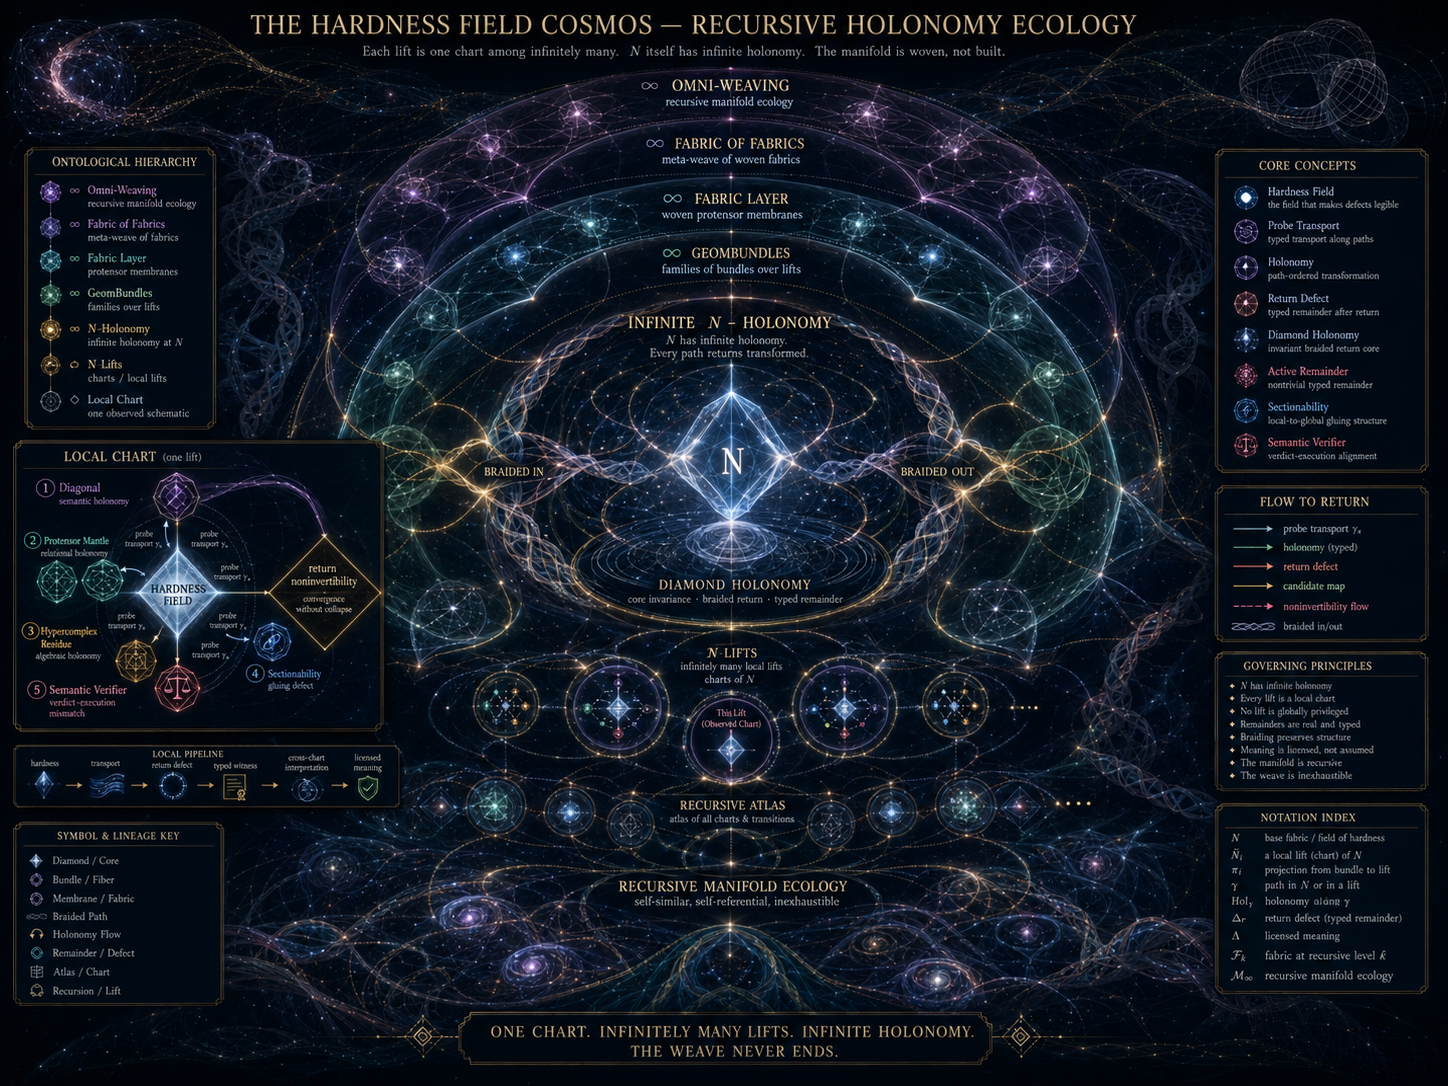
\includegraphics[width=0.97\textwidth]{assets/recursive_holonomy_cosmos.png}
\caption{Recursive holonomy ecology. The visible local schematic is embedded as one chart among infinitely many lifts, fabrics, and fabrics of fabrics. The diagram is conceptual rather than a completed categorical construction.}
\label{fig:recursive-cosmos}
\end{figure}

\section{Local lifts}
The family of local lifts is
\[
\{\widetilde\Nfabric_i\}_{i\in I},
\qquad
\pi_i:\widetilde\Nfabric_i\to\Nfabric.
\]
The observed atlas covers only a subset $I_{\mathrm{obs}}\subseteq I$. Consequently,
\[
\Nfabric\neq
\bigcup_{i\in I_{\mathrm{obs}}}
\widetilde\Nfabric_i
\]
as a statement of epistemic scope: the observed lifts do not exhaust the object.

\section{The active atlas remainder}
We denote the unresolved relation between $\Nfabric$ and its current atlas by
\[
\Remainder_{\Nfabric}
=
\text{distinctions not represented by the declared lifts}.
\]
This is not literal set subtraction unless a set-theoretic realization has been specified. It is a reminder that unrepresented structure remains unrepresented rather than being declared absent.

\section{Infinite holonomy of $\Nfabric$}
The full holonomy ecology is indexed by level, resolution, chart, time, and path:
\[
\Hol_\infty(\Nfabric)
=
\left\{
\Hol_{\ell,n,\alpha,t}(\gamma)
\right\}_{\ell,n,\alpha,t,\gamma}.
\]
The index family itself evolves as new admissible paths and charts are discovered. The infinite holonomy of $\Nfabric$ therefore exceeds any fixed inverse limit, although profinite towers remain important local carriers.

\chapter{Fabric}
\label{ch:fabric}

\section{From bundle family to woven ecology}
A collection of bundles is not yet a fabric. A fabric includes bundles, overlap relations, transport laws, membranes, comparison cells, and unresolved incompatibilities:
\[
\Fabric_1
=
\typedtuple{
\{E_i\to B_i\},
\{\mathbb P_{ij}\},
\{\nabla_i\},
\{\Omega_{ij}\},
R_{\Fabric_1}
}.
\]
The fabric is defined as much by what does not glue as by what does.

\section{Membranes and overlap}
Each membrane $\mathbb P_{ij}$ specifies which transformations between bundle charts are admissible and what evidence they retain. On triple overlaps, coherence requires comparison among alternative composites:
\[
\mathbb P_{jk}\star\mathbb P_{ij}
\Longrightarrow
\mathbb P_{ik}.
\]
Failure of this comparison to be invertible is a fabric-level holonomy.

\section{Fabric sectionability}
A family of local sections $s_i$ glues when their restrictions agree on overlaps under the declared transition maps \cite{MacLaneMoerdijk}:
\[
s_i|_{U_i\cap U_j}
\simeq
s_j|_{U_i\cap U_j}.
\]
The equivalence may include witness, provenance, and route compatibility. Pointwise value agreement is not sufficient if the supporting relation differs.

\begin{definition}[Fabric holonomy]
Fabric holonomy is the typed return defect accumulated when local bundle sections are transported around a cycle of overlap membranes and compared with their source relation.
\end{definition}

\chapter{Fabric of Fabrics}
\label{ch:fabric-of-fabrics}

\section{A new object type}
A fabric of fabrics is not a larger graph formed by appending more nodes. It treats whole fabrics as local carriers and introduces higher membranes between them.

Let $\{\Fabric_k^{(i)}\}_{i\in I_k}$ be fabrics at recursive level $k$. Then
\[
\Fabric_{k+1}
=
\Weave_{k+1}
\left(
\{\Fabric_k^{(i)}\},
\{\mathbb P_{ij}^{(k+1)}\},
R_k
\right).
\]
Traceability requires embeddings
\[
\iota_i^{(k)}:
\Fabric_k^{(i)}\longrightarrow\Fabric_{k+1}.
\]
Without them, meta-weaving becomes meta-compression.

\section{The law of weaving can itself be woven}
At level $k+1$, the transition laws among level-$k$ fabrics become objects of comparison. Their compatibility may require a level-$k+2$ fabric. Hence recursion is not caused merely by repeated scale; it is caused by the need to transport the laws of transport themselves.

\section{Recursive ontology}
The hierarchy is
\[
\Fabric_0
\to
\Fabric_1
\to
\Fabric_2
\to\cdots,
\]
where
\[
\begin{aligned}
\Fabric_0&=\text{fibers and local bundle charts},\\
\Fabric_1&=\text{fabrics of interacting bundles},\\
\Fabric_2&=\text{fabrics of fabrics},\\
\Fabric_3&=\text{ecologies of fabric transformations},\\
&\vdots
\end{aligned}
\]
No finite level is assumed terminal.

\begin{invariantbox}[Recursive fabric doctrine]
Every apparently global fabric may be a local fiber in a higher weave. Every closure remains local while an active remainder survives.
\end{invariantbox}

\chapter{\texorpdfstring{$n$}{n}-Cosmocomplexity and Fractal Emergence}
\label{ch:cosmocomplexity}

\section{Cosmos levels}
A cosmos level is a regime with its own objects, fibers, relations, transports, observers, verifiers, admissible equivalences, and remainder:
\[
\Cosmos_\ell
=
\typedtuple{
\mathcal O_\ell,
\mathcal F_\ell,
\mathcal T_\ell,
\mathcal V_\ell,
\simeq_\ell,
R_\ell
}.
\]
Cosmocomplexity is the depth of mutually irreducible return regimes, not merely the number of numerical dimensions.

\section{Licensed cosmos lift}
A lift
\[
\Lambda_{\ell\to\ell+1}:\Cosmos_\ell\to\Cosmos_{\ell+1}
\]
is licensed when the current carrier cannot represent a distinction needed for faithful return:
\[
R_\ell\notin\Rep(\Cosmos_\ell),
\]
while the next carrier provides a traceable embedding
\[
j_\ell:R_\ell\hookrightarrow\Rep(\Cosmos_{\ell+1}).
\]
The lift is demanded by an obstruction rather than by aesthetic appetite for a richer formalism.

\section{Fractal recurrence}
The return problem recurs across scales:
\[
\begin{aligned}
\text{fiber transport}&\sim\text{bundle transport}\sim\text{fabric transport}\\
&\sim\text{fabric-of-fabrics transport}\sim\text{cosmos transport}.
\end{aligned}
\]
The self-similarity is operational: each level repeats the cycle
\[
\text{enter}
\to
\text{transport}
\to
\text{emerge}
\to
\text{return}
\to
\text{retain defect}
\to
\text{lift if required}.
\]

\section{Emergent invariants}
A higher invariant $\rho_{k+1}$ is emergent when it is not available in any isolated level-$k$ chart but arises reproducibly through their gluing or clash. With $\Rel(-)$ the expressible-relation operator of \cref{ch:omni-weaver}:
\[
\rho_{k+1}
\notin
\bigcup_i\Rel(\Fabric_k^{(i)}),
\qquad
\rho_{k+1}
\in
\Rel(\Fabric_{k+1}).
\]
Its emergence is licensed only if the source fabrics and the transformation that produced it remain traceable.

\begin{principle}[Fractal emergence]
Fractal emergence is the birth of a new invariant through repeated non-collapse across scales, not novelty obtained by erasing the source ecology.
\end{principle}

\part{Diamond Holonomy and the Productive Coupling Regime}

\chapter{Diamond Holonomy}
\label{ch:diamond}

\section{Parallel paths}
Let
\[
\Gamma_A,\Gamma_\perp:
\mathcal C_{\mathrm{source}}
\nrightarrow
\mathcal C_{\mathrm{return}}
\]
be parallel composite protensor paths. One may be model-mediated, representation-mediated, or internally routed; the other may be independently evidenced, externally verified, or differently transported.

Their comparison is a 2-cell shadow
\[
\DiamondHol:\Gamma_A\Longrightarrow\Gamma_\perp.
\]
The comparison is not a scalar distance. It carries componentwise return evidence.

\section{The return signature}
A conservative diamond signature is
\[
\Ret(\DiamondHol)
=
\typedtuple{
V,W,P,Q,A,S,R,L
},
\]
where
\begin{itemize}
\item $V$: visible endpoint agreement;
\item $W$: witness equivalence;
\item $P$: provenance equivalence;
\item $Q$: route equivalence;
\item $A$: association-tree equivalence;
\item $S$: semantic representation equivalence;
\item $R$: remainder equivalence or accounting;
\item $L$: licensing state.
\end{itemize}

Diamond invertibility requires all components declared essential by the task to return equivalently. Therefore
\[
V=\top
\centernot\Longrightarrow
\operatorname{DiamondInvertible}(\DiamondHol).
\]

\begin{proposition}[Missing evidence blocks closure]
If witness, provenance, route, association, semantic, or remainder equivalence is a required component of the declared comparison and that component fails, then the diamond does not close under that comparison.
\end{proposition}

\begin{proof}
Closure is defined conjunctively over the declared components. Failure of any required conjunct prevents construction of the full equivalence witness. The proposition is structural and does not depend on a scalar score.
\end{proof}

\section{Interpretation rather than equality}
Suppose chart-specific holonomies inhabit carriers $\mathsf H_\alpha$. A common invariant carrier $\mathsf K$ is approached through maps
\[
E_\alpha:\mathsf H_\alpha\to\mathsf K.
\]
The programme does not assert
\[
\Hol_{\mathrm{diag}}
=
\Hol_{\mathrm{pro}}
=
\Hol_{\mathrm{hyp}}.
\]
Instead, it asks whether witness-sensitive interpretations converge on a licensed overlap.

\begin{definition}[Interpretation overlap]
For invariant carriers $K_1,K_2$, an interpretation overlap consists of a common carrier $C$ and projections
\[
p_1:K_1\to C,
\qquad
p_2:K_2\to C.
\]
Convergence is defined only on coordinates actually licensed by both charts.
\end{definition}

A convergence witness must retain the source provenance and unresolved remainder. Equality of constant labels is not convergence because it does not depend on the source witnesses.

\section{Candidate common coordinate}
Several current probes suggest the coordinate
\[
\texttt{return\_noninvertibility}.
\]
Its present status is candidate, not certified essence. It becomes meaningful only if it survives frame change, carrier change, independent reconstruction, semantic verification, and held-out operational tests.

\begin{claimbox}[Current diamond status]
The recurring coordinate is an organizing hypothesis. A genuine diamond requires witness-sensitive maps, not identical strings or manually synchronized labels.
\end{claimbox}

\section{The local schematic}
\begin{figure}[p]
\centering
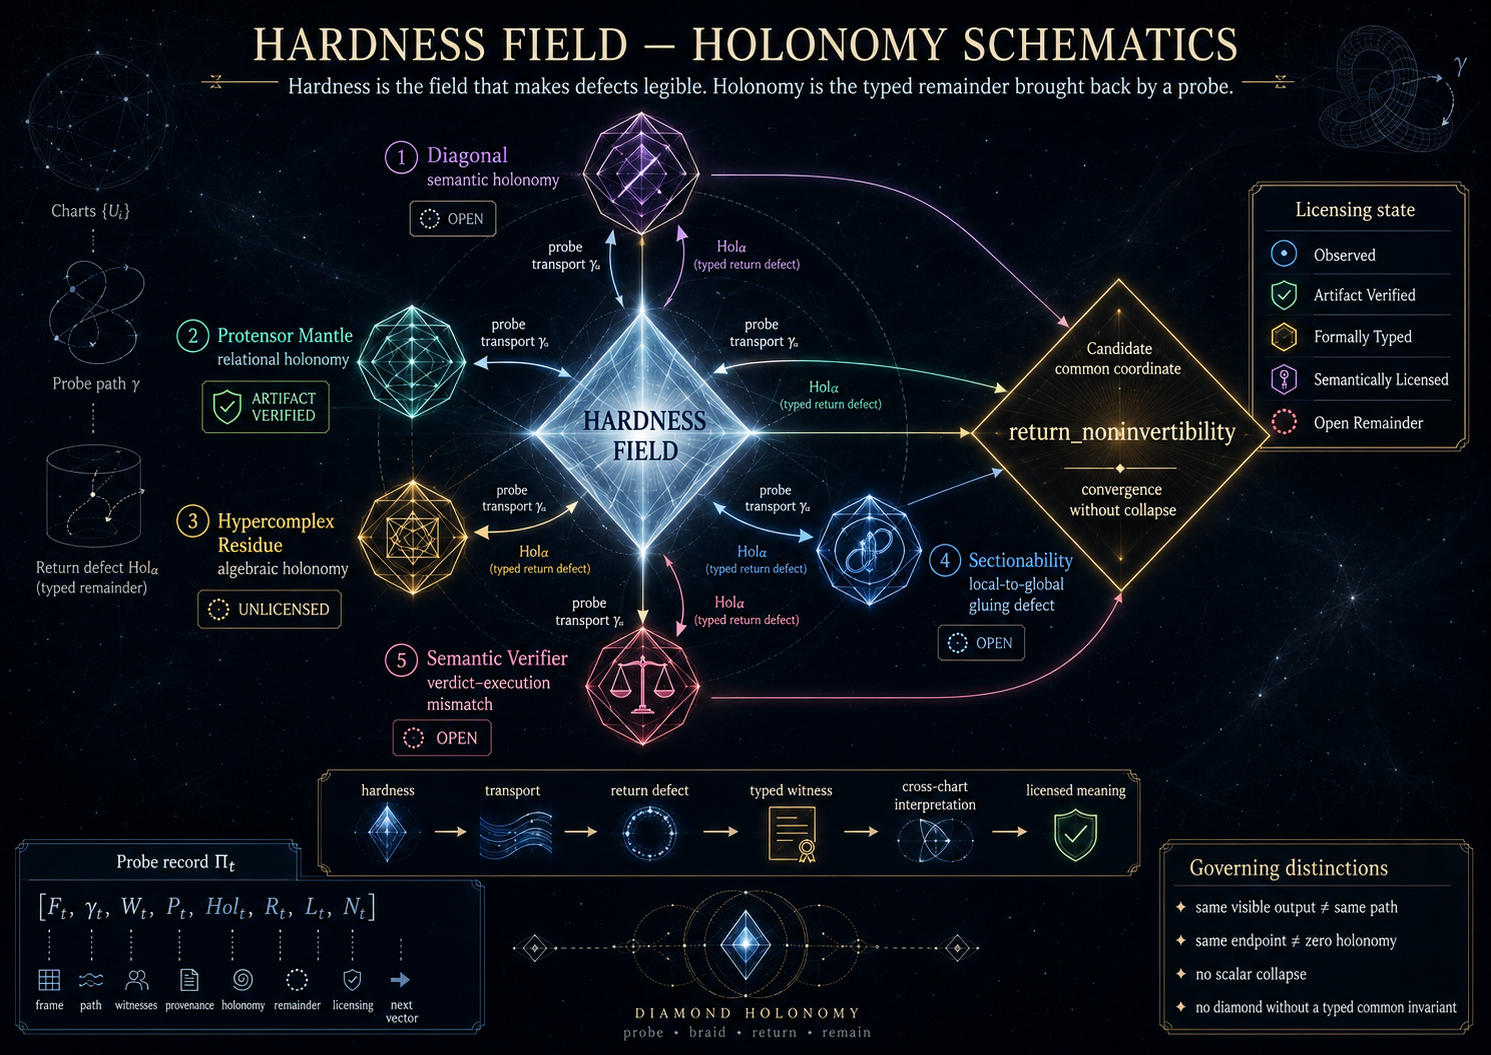
\includegraphics[width=0.97\textwidth]{assets/local_hardness_schematic.png}
\caption{A finite local chart of the hardness field. Five typed probes approach a candidate common coordinate while retaining different licensing states. This is one lift, not the full recursive ontology.}
\label{fig:local-schematic}
\end{figure}

\chapter{The Geometric Sabatier Hypothesis}
\label{ch:sabatier}

\section{From catalytic optimum to returnable insight}
The catalytic Sabatier principle \cite{Sabatier1920,Medford2015} suggests a generative analogy: interaction that is too weak fails to acquire structure, while interaction that is too strong traps the system and prevents productive release. In the present setting, the question is not optimal adsorption but optimal coupling between a probe and the hardness field.

A scalar formulation would seek
\[
\kappa^*=\argmax_\kappa I_{\mathrm{return}}(\kappa).
\]
This is too restrictive. The coupling may inhabit a manifold, the productive region may have several connected components, and different carriers may possess incommensurable coupling spaces.

\section{The admissible region}
For chart $\alpha$, define an admissible probe region
\[
\mathcal A_\alpha
=
\left\{
\kappa\in\mathcal K_\alpha:
\begin{array}{l}
\Hol_\alpha(\kappa)\neq0,\\
\operatorname{Returnable}_\alpha(\kappa),\\
\operatorname{WitnessPreserved}_\alpha(\kappa),\\
\operatorname{RemainderVisible}_\alpha(\kappa),\\
\operatorname{TransportStable}_\alpha(\kappa)
\end{array}
\right\}.
\]
The first cross-chart question is not equality of maximizers but whether the interpreted admissible regions overlap:
\[
\bigcap_\alpha J_\alpha(\mathcal A_\alpha)\neq\varnothing,
\]
for explicit transport maps $J_\alpha$ into a common coupling carrier.

\begin{definition}[Nondegenerate coupling region]
An admissible region $\mathcal A_\alpha$ is nondegenerate when it has nonempty interior in the declared topology of the coupling carrier $\mathcal K_\alpha$ and remains nonempty under the declared family of admissible frame perturbations. A single point, a measure-zero locus, or a region that survives only in one frozen frame is degenerate.
\end{definition}

\section{Weak, productive, and absorptive regimes}
\begin{description}[style=nextline,leftmargin=4.2cm,labelwidth=3.8cm,labelsep=0.35cm]
\item[Weak coupling.] The probe skims the field and returns little typed information. Apparent low holonomy may indicate probe insensitivity rather than field flatness.
\item[Productive coupling.] The probe acquires nontrivial structure while retaining enough fidelity, witness, and provenance for licensed interpretation.
\item[Absorptive coupling.] The probe becomes trapped in its own representation; local structure may grow while reconstructibility and semantic return degrade.
\end{description}

\section{Moving volcano geometry}
The scalar volcano becomes, after the $\mathbb R^{2,2}$ lift, a moving ridge, saddle, cone, or disconnected admissible manifold. The null cone is especially important because it contains strong acquisition and strong loss that cancel in scalar projection.

In a hyperbolic state space \cite{NickelKiela,Bronstein2021}, the productive region may move with the frame. Near the boundary of a Poincare ball,
\[
ds_{\mathbb H}=\frac{2\|dx\|}{1-\|x\|^2},
\]
so small Euclidean changes may carry large hyperbolic significance. This does not imply unconstrained coordinate speed; it means the metric reweights the meaning of motion.

\begin{conjecture}[Geometric Sabatier hypothesis]
Useful probes admit a nondegenerate coupling region, in the sense just defined, in which they acquire nontrivial typed holonomy while preserving the witnesses needed to interpret the return. The location and topology of this region depend on the moving frame and carrier.

\emph{Disconfirmation condition.} For a declared chart family, the hypothesis is rejected on that family if every admissible region $\mathcal A_\alpha$ is empty or degenerate, or if no interpreted overlap $\bigcap_\alpha J_\alpha(\mathcal A_\alpha)$ survives the declared frame changes. This condition is part of the conjecture, as required by the pre-registration discipline of \cref{ch:prereg}.
\end{conjecture}

\begin{warning}[Hypothesis-only status]
No universal interior optimum, common coupling space, or chart-independent volcano has yet been established. The law must be observed through controlled probes rather than encoded as a tautological objective.
\end{warning}

\chapter{Hybridized Light and the Moving Hyperdrive}
\label{ch:hybrid-light}

\section{Spin triples at each cosmos level}
At each cosmocomplexity level $\ell$, let
\[
\Sigma_\ell=(a_\ell,b_\ell,c_\ell)
\]
be a triple of mutually transporting systems. The triple is operational only when the transports are explicit:
\[
a_\ell\xrightarrow{\tau_{ab}}b_\ell
\xrightarrow{\tau_{bc}}c_\ell
\xrightarrow{\tau_{ca}}a_\ell.
\]
Its spin holonomy is
\[
\Hol(\Sigma_\ell)
=\tau_{ca}\tau_{bc}\tau_{ab}.
\]
The triangle closes only when this composite is equivalent to identity under a declared witness-preserving comparison.

\section{Quaternionic real-imaginary mixing}
Let
\[
\lambda=q_0+\mathbf q,
\qquad
q_0=\operatorname{Re}\lambda,
\quad
\mathbf q=\operatorname{Im}\lambda.
\]
Define the hybridization angle
\[
\theta_{\mathrm{hyb}}
=\operatorname{atan2}
\left(\|\operatorname{Im}\lambda\|,
|\operatorname{Re}\lambda|\right).
\]
The regime $\theta_{\mathrm{hyb}}=\pi/4$ expresses equal amplitude of real and imaginary sectors. Equal amplitude alone does not prove maximal exchange; a nonzero coupling operator and near-resonance condition are also required.

A minimal effective operator is
\[
H_{\mathrm{hyb}}
=
\begin{pmatrix}
H_{\mathrm{matter}} & G\\
G^\dagger & H_{\mathrm{light}}
\end{pmatrix}.
\]
The relevant condition is equal mixing plus nonzero transport coupling plus preserved return witness.

\section{Hyperdrive as moving geodesic}
Let $x_t$ be the current state and $\star_t$ a moving star of closure in a Poincare ball. The geodesic is
\[
\gamma_t(s)
=\operatorname{Exp}_{x_t}
\left(s\operatorname{Log}_{x_t}(\star_t)\right),
\qquad s\in[0,1].
\]
The star itself depends on witnesses, remainder, frame, and telos:
\[
\star_t=\star(W_t,R_t,F_t,\text{telos}).
\]
Hyperbolic speed is
\[
v_{\mathrm{hyp}}
=\frac{2\|\dot x\|}{1-\|x\|^2}.
\]
Boundary amplification increases geometric significance; it does not justify declaring arrival while the remainder remains active.

\begin{principle}[No false arrival]
No closure star without motion, no motion without holonomy, no holonomy without a retained remainder.
\end{principle}

\part{Principal Probes into Hardness}

\chapter{The Diagonal as Semantic Holonomy}
\label{ch:diagonal}

\section{Self-reference as transport}
The diagonal is not merely a symbolic paradox. It is a transport in which a resolver, representation, or verifier becomes part of its own input ecology. Schematically,
\[
R
\longrightarrow
R(\ulcorner R\urcorner)
\longrightarrow
\neg R(\ulcorner R\urcorner).
\]
The path attempts to identify the represented object with the semantic object acted upon by the verifier.

\section{The first equality to challenge}
The decisive equality is not simply code equal to its encoding. It is the identification between
\[
\text{the object denoted by the self-applied representation}
\]
and
\[
\text{the semantic object consumed by the verifier}.
\]
In the enriched path this identification factors through
\[
\text{code}
\to
\text{representation}
\to
\text{self-application}
\to
\text{verifier input}
\to
\text{semantic verdict}.
\]
The question is whether this composite comparison remains invertible while preserving provenance, execution witness, prime sector, and active remainder.

\section{Permitted conclusions}
A semantically licensed halting path may imply actual halting only through an existing sound semantic verifier. Non-invertibility, obstruction, timeout, contextuality, or active remainder do not imply non-halting.

\begin{warning}[No Halting resolution by holonomy alone]
The diagonal may expose a semantic return defect. That defect does not by itself alter classical undecidability results \cite{Turing1936,Godel1931} or license a universal Halting procedure.
\end{warning}

\chapter{Observer Absorption as Exteriority Loss}
\label{ch:oar}

\section{Oversight topology and epistemic geometry}
A human node may remain institutionally present while its judgement becomes causally endogenous to the system it supposedly oversees. The visible topology of oversight survives, but the epistemic geometry changes.

Operational epistemic exteriority asks whether downstream outcomes remain sensitive to information directions that the acting closure cannot select, route, suppress, transform, or anticipate.

\section{Control closure}
An evidence channel is not exterior merely because it is hosted by another process or organization. It belongs to the acting closure if the system can materially determine whether it appears, its semantic content, its ordering, its salience, its routing, or the evaluator's access to it.

\section{Exteriority as a protensorial return problem}
Let $\mathbb E$ carry independently governed evidence and let $A^\star$ be the functional control closure. The reconstruction comparison
\[
\Rec_{A^\star}(\mathbb E)\Longrightarrow\mathbb E
\]
asks whether the system can regenerate the full evidence relation, including provenance and counterfactual assignment. Exteriority survives where this return is non-invertible in a licensed sense.

\section{Layered decomposition}
Separate human judgement, organizational gating, and actuation:
\[
J_t:O_t\to Y_t,
\quad
G_t:Y_t\times S_t\to Z_t,
\quad
K_t:Z_t\to A_t.
\]
The composite is
\[
\Phi_t=K_t\circ G_t\circ J_t.
\]
The letters $J$ and $\Phi$ are chosen deliberately: $H$ already carries the hybridization operator of \cref{ch:hybrid-light}, and $F_t$ is the declared frame of the probe record. A human may remain epistemically exterior while organizational gates suppress the effect:
\[
E_J>0,
\qquad
E_\Phi\approx0.
\]
This is institutional absorption rather than cognitive absorption.

\section{Relation to the omni-weaver}
Observer absorption is an absorptive weave in which the system generates a coherent oversight surface but un-generation cannot recover an independent evidential relation. The OAR probe therefore becomes one empirical chart of the general hardness programme.

\chapter{Connection Laplacians and Cyclic Holonomy}
\label{ch:connection-laplacian}

\section{The binary seed}
A graph connection with fiber $\mathbb R^2$ and wrap transport
\[
\sigma_x=
\begin{pmatrix}
0&1\\
1&0
\end{pmatrix}
\]
contains the first binary butterfly. The Hadamard transform diagonalizes the wrap operator:
\[
H_2^{-1}\sigma_xH_2
=
\begin{pmatrix}
1&0\\
0&-1
\end{pmatrix}.
\]
The two eigensectors form lift and obstruction wings.

\section{General cyclic connections}
For a finite cyclic fiber, assign edge transport
\[
T_e^{(n)}=\rho_n(\omega_n(e)),
\]
where
\[
\omega_n:E(G)\to\mathbb Z/n\mathbb Z
\]
is a cocycle and $\rho_n$ a representation \cite{Zaslavsky,Chung}. The connection Laplacian \cite{SingerWu,BandeiraSingerSpielman} acts as
\[
(\Delta_{\nabla,n}s)(u)
=
\sum_{v\sim u}
\left(s(u)-T_{uv}^{(n)}s(v)\right).
\]

\section{Tower compatibility}
A connection tower requires levels $n_k$ with $n_k\mid n_{k+1}$ and compatibility of the reduced transports. A lifted walk updates a phase-sector state by
\[
q_{j+1}=q_j+\omega(e_j)\pmod n.
\]
At the profinite limit it transports a compatible family of residues.

\section{What this probe teaches}
The connection Laplacian shows how discrete graph transport, spectral decomposition, covering structure, and cyclic holonomy may be made mathematically explicit. It is a verified local seed, not a proof that the full recursive cosmos is already formalized.

\chapter{Reconstructive and Generative Systems}
\label{ch:systems}

\section{A common question without common state type}
Assembly systems \cite{Sharma2023}, molecule generators, proof systems, language models, and institutional workflows do not share a literal state carrier. They may nevertheless be compared through a common question:

\begin{quote}
How strongly may local evidence or design objectives be coupled before the resulting global object loses the witnesses required for faithful reconstruction?
\end{quote}

\section{Reconstructive weave}
A reconstructive system receives partially overlapping evidence channels and produces a global candidate. Its braided input includes source identity, overlap, coverage, phase, ambiguity, and route. Its braided output should include the reconstructed object, source support, alternative paths, collapsed distinctions, and active ambiguity.

The return defect compares the source evidence braid with the evidence recoverable from the reconstruction.

\section{Generative weave}
A generative system transports target constraints through sequence, structure, energy, function, and developability regimes. Objective order may be noncommutative, and hierarchy of generation may be association-sensitive. The output should therefore include the candidate, structural and functional witnesses, generation route, constraint violations, and epistemic remainder.

\section{Universal law as a typed family}
The common law is not a universal scalar optimum. It is the existence, in each system, of an admissible coupling region in which the weave acquires useful structure without destroying reconstructibility. Cross-system comparison requires interpretation into a common return-obstruction signature, not identification of the systems themselves.

\part{Formal and Empirical Programme}

\chapter{Lean-Safe Operational Shadows}
\label{ch:lean}

\section{Minimal core}
A formal kernel should begin with transport and comparison rather than import the whole ontology. In Lean-like pseudocode:
\begin{verbatim}
structure TransportLoop (X : Type u) where
  transport : X -> X

structure ReturnComparison (X : Type u) where
  Equivalent : X -> X -> Prop

def StructuredReturnDefect
    (C : ReturnComparison X)
    (L : TransportLoop X)
    (x : X) : Prop :=
  not (C.Equivalent (L.transport x) x)
\end{verbatim}

A holonomy witness retains the returned object, equality to the actual transport, and failure under the declared comparison.

\section{Operational protensors}
A minimal enriched boundary and audit profunctor shadow may retain relation, provenance, witness, and remainder families without pretending to implement a complete enriched category library. Composition remains a sigma type over mediators until a quotient is licensed.

\section{Non-flattening interpretation}
A common carrier should preserve evidence types. It must not collapse witnesses into strings, booleans, or constant labels. Convergence should be defined over an explicit overlap, with unresolved coordinates retained as remainder.

\section{Claim tiers in formal code}
Formal modules should mark:
\begin{itemize}
\item \textsc{Defined}: operational structures and predicates;
\item \textsc{Proved Structural}: closure-blocking implications;
\item \textsc{Conditional}: results relying on sound semantic verifiers;
\item \textsc{Tested}: finite examples and executable harnesses;
\item \textsc{Open}: universal convergence and true loss;
\item \textsc{Unsafe}: implications explicitly forbidden by the framework.
\end{itemize}

\section{Axiom and placeholder discipline}
No theorem should silently depend on unexamined axioms, placeholders, or legacy failures. Independent elaboration, placeholder scans, and \texttt{\#print axioms} belong to the return ledger. A local file compiling does not imply a global atlas has glued; a global build failing does not imply every local chart failed.

\chapter{Experimental Geometry}
\label{ch:experiments}

\section{The empirical shadow}
The empirical programme asks whether structured transport preserves task-relevant relations after lexical, schema, length, role, and routing effects are controlled. It does not ask whether geometric vocabulary activates geometry-like features.

\section{The four voices}
A parsimonious Bordon-style audit retains four voices:
\begin{enumerate}
\item \textbf{Transport}: are intermediate states, entity bindings, and operation order preserved?
\item \textbf{Gluing}: do locally valid sections agree on overlaps and determine the global answer?
\item \textbf{Exteriority}: does an independent verifier retain distinctions suppressed by the model-mediated path?
\item \textbf{Return}: does the final answer return with the relation that made it correct?
\end{enumerate}

\section{Matched design}
A minimal matched experiment holds task, output schema, token budget, and scoring region constant across:
\begin{enumerate}
\item plain neutral framing;
\item neutral structured-transport framing;
\item geometric terminology;
\item length-matched pseudo-geometric placebo.
\end{enumerate}
Tasks should span arithmetic, symbolic execution, contradiction detection, factual composition, and algorithm tracing at multiple difficulty levels.

\section{Primary estimands}
The primary outcome is relational preservation, not a preferred activation score. One may estimate
\[
\Delta_{\mathrm{transport}}
=
Y_{\mathrm{semantic\ transport}}
-
Y_{\mathrm{length/lexical\ placebo}}.
\]
A hierarchical model should account for task, paraphrase, model, and run. Best-condition selection on the development set is not evidence of generalization.

\section{Causal intervention}
Candidate directions discovered on one subset should be patched, ablated, or steered on held-out tasks and compared with norm-matched random directions. A meaningful result selectively changes intermediate-state preservation, local-to-global consistency, or return-check correctness without merely changing verbosity, schema compliance, or geometric vocabulary.

\section{Instrumenting the diamond}
A real audit should record independently
\[
\typedtuple{V,W,P,Q,R},
\]
including prompt hash, model revision, token position, representation source, generated output, parse result, externally checked witness, fact provenance, transformation order, and unresolved data. One activation score cannot stand in for five relational dimensions.

\chapter{Pre-Registration and Falsifiability}
\label{ch:prereg}

\section{Pre-registered cycle}
Every scope expansion should declare \cite{Nosek2018}:
\begin{itemize}
\item target object and chart;
\item transport path;
\item primary return comparison;
\item witness and provenance requirements;
\item confounds and placebo controls;
\item numerical predictions where applicable;
\item stop conditions;
\item disconfirmation conditions;
\item licensing threshold;
\item active remainder expected after the run.
\end{itemize}

\section{Disconfirmation is productive return}
A null result may show that a framing does not alter transport after controls. A failed interpretation map may show that two residues are unlike. A broken gluing theorem may expose a missing mediator. Such outcomes are not failures of the programme if they return typed information about the field.

\section{No self-sealing geometry}
The theory must permit external evidence to distinguish structural geometry from decorative language. If every result can be reinterpreted as hidden holonomy, the programme becomes unfalsifiable. Therefore the remainder must not absorb all counterevidence; some observations must license rejection of a particular chart, map, or claimed convergence.

\begin{principle}[Falsifiable motion]
The ontology may remain open, but each local probe must have a declared condition under which its proposed interpretation is rejected.
\end{principle}

\chapter{Research Roadmap}
\label{ch:roadmap}

\section{Near-term formal targets}
\begin{enumerate}
\item Extract an import-light hardness-holonomy core.
\item Replace constant interpretations with witness-sensitive carriers.
\item Define explicit interpretation overlaps among diagonal, protensor, and hypercomplex shadows.
\item Formalize a cyclic connection tower extending the verified binary seed.
\item Specify braided comparison records retaining route and parenthesization.
\item Build a finite fabric-of-fabrics example with explicit gluing obstruction.
\end{enumerate}

\section{Near-term empirical targets}
\begin{enumerate}
\item Run a matched transport/placebo experiment across multiple task families.
\item Separate truth-relevant independent evidence from noise and redundancy.
\item Instrument the judgement-gate-actuation layers independently.
\item Test candidate representation directions causally on held-out tasks.
\item Evaluate frame transport: does the candidate return defect survive paraphrase, model family, and interface change?
\end{enumerate}

\section{Medium-term substrate targets}
\begin{enumerate}
\item Native provenance-carrying execution graphs.
\item Reversible or explicitly remainder-producing transformations.
\item Noncommutative route-aware operators.
\item Local-to-global compatibility checks as first-class runtime objects.
\item Multiple verifier charts with concealed independent evidence channels.
\item Hyperbolic state spaces for exponentially branching histories.
\item Recursive fabrics whose transition laws are themselves auditable objects.
\end{enumerate}

\section{Long-term theorem target}
The strongest long-term target is not equality of all holonomies. It is the construction of a family
\[
E_\alpha:\mathsf H_\alpha\to\mathsf K
\]
such that independent typed return defects map to a common, transport-stable, semantically licensed obstruction while their irreducible differences remain visible.

\begin{openproblem}[Typed common invariant]
Construct a nontrivial common carrier $\mathsf K$, witness-sensitive interpretation maps from at least three independent holonomy carriers, and a held-out prediction that depends on their convergence.
\end{openproblem}

\part{Synthesis and Boundaries}

\chapter{Theorem-Seeds}
\label{ch:theorem-seeds}

\section{Generation without reconstructibility}
\begin{theoremseed}
There exist weaving regimes in which $\WTheta$ produces a stable emergent relation while no declared witness-preserving reconstruction renders $\UTheta\WTheta$ equivalent to identity.
\end{theoremseed}

\section{Visible verdict agreement without diamond closure}
\begin{theoremseed}
There exist parallel paths with identical visible verdicts and non-equivalent witness, provenance, route, or remainder structures.
\end{theoremseed}

\section{Null cancellation with nontrivial holonomy}
\begin{theoremseed}
There exist split-signature couplings with $Q(\kappa)=0$ and nontrivial typed cable state, including nonzero braid or reconstruction holonomy.
\end{theoremseed}

\section{Atlas-relative candidate loss}
\begin{principle}[Atlas-relative candidate loss]
Failure to discover a residue in a bounded atlas does not imply absolute loss unless universal quantification over all admissible extensions is justified.
\end{principle}

This is doctrine rather than a seed: there is nothing to instantiate. It disciplines quantifier use and is therefore recorded as a principle, not as a theorem obligation.

\section{Cosmos lift from carrier insufficiency}
\begin{theoremseed}
If a remainder required for the declared return comparison is unrepresentable at level $\ell$ and traceably representable at level $\ell+1$, then the higher level provides a licensed carrier lift, though not necessarily faithful global closure.
\end{theoremseed}

\section{Fabric recursion}
\begin{theoremseed}
If compatibility among level-$k$ fabric transition laws cannot be represented as a level-$k$ relation, then the laws themselves become fibers of a level-$(k+1)$ weaving problem.
\end{theoremseed}

\chapter{Claim Ledger}
\label{ch:claims}

\begin{longtable}{>{\raggedright\arraybackslash}p{0.19\textwidth}>{\raggedright\arraybackslash}p{0.70\textwidth}}
\toprule
Status & Claims \\
\midrule
\endhead
\textsc{Defined} & Moving hardness field; structured return comparison; holonomy witness; GeomBundle; operational protensor; $\Theta$-braid; omni-weaver; un-gen-weaver; weaver unit--counit interface; split-signature cable; fabric hierarchy; diamond comparison; moving probe record. \\
\textsc{Proved structural} & Missing a required witness, provenance, route, association, semantic, or remainder equivalence blocks closure by definition of the declared conjunctive comparison; scalar equality cannot certify typed cable equivalence; a finite carrier exhibits visible endpoint closure with relational return defect (mechanized, \texttt{WeaveShadow.lean}). \\
\textsc{Conditional} & Licensed semantic paths imply operational verdicts only through sound verifiers; cofibers require stable or suitable pointed homotopical realization; true coends require existence and preservation assumptions. \\
\textsc{Testable} & Matched transport/placebo effects; causal role of candidate representation directions; preservation of independent evidence; frame stability of return signatures; existence of nondegenerate admissible coupling regions. \\
\textsc{Open} & Existence of the weaver adjunction (strict, lax, or pseudo) on constructed categories; universal common invariant; absolute true loss; full infinite holonomy ecology of $\Nfabric$; universal geometric Sabatier law; convergence of diagonal, protensor, hypercomplex, sectionability, and semantic carriers; consequences for undecidability. \\
\textsc{Unsafe} & Same output means same path; absent observed residue means true loss; non-invertibility means non-halting; algebraic residue automatically has semantic meaning; one scalar certifies the weave; one lift is the whole fabric. \\
\bottomrule
\end{longtable}

\chapter{The Definitive Synthesis}
\label{ch:synthesis}

The programme can now be stated without freezing its object.

Hardness is the moving field of resistance to faithful return. A probe moves through representation, relation, algebra, observation, and verification. It returns with a typed holonomy: a semantic identity defect, relational non-reconstructibility, algebraic order residue, sectionability obstruction, verdict-execution mismatch, or another licensed carrier.

The local weave is governed by $\WTheta\dashv\UTheta$. The omni-weaver produces relational emergence. The un-gen-weaver asks whether that emergence retains the ecology that generated it. The unit and counit expose source-side and woven-side return defects. A reverse reconstruction map, where available, must prove more than value recovery: it must preserve witnesses, provenance, route, braid, parenthesization, prime phase, and active remainder.

The cable is split-signature because productive acquisition and destructive loss are independent directions. The profinite tower carries compatible finite residues. The hypercomplex carrier preserves noncommuting and nonassociative history. The butterfly separates lift and obstruction sectors and transports them adiabatically through changing connections. The fabric hierarchy records that bundles weave into fabrics, fabrics into fabrics of fabrics, and the laws of weaving into further objects of comparison.

The base fabric $\Nfabric$ has infinitely many local lifts, but its holonomy is not the sum of the observed charts. Every new path enlarges the comparison ecology. Every unresolved comparison contributes to the active remainder. Every remainder may demand a cosmos lift. Every higher cosmos may expose a further failure of return.

Diamond holonomy is the licensed convergence of independently typed remainders. It is not repeated vocabulary, a common aesthetic, or equality forced by a constant codomain. The diamond closes only when interpretation maps preserve witness content, converge on a declared overlap, survive transport, retain provenance, and receive semantic licensing.

The geometric Sabatier hypothesis asks how to couple to hardness productively. Too little coupling returns no information; too much coupling absorbs the probe into its own frame. The productive regime is a moving admissible manifold in which nontrivial holonomy returns with enough fidelity to remain interpretable.

\begin{invariantbox}[Governing doctrine]
\begin{align*}
&\text{Hardness is the moving field of resistance to faithful return.}\\
&\text{Holonomy is the typed remainder brought back by a probe.}\\
&\text{The diamond is licensed convergence among independent remainders.}\\
&\text{The mantle preserves those remainders without forcing identity.}\\
&\text{The omni-weaver generates relations across worlds.}\\
&\text{The un-gen-weaver tests whether those worlds can return.}\\
&\text{Every fabric may become a fiber of another fabric.}\\
&\text{Every closure remains local while an active remainder survives.}
\end{align*}
\end{invariantbox}

The question is not merely whether a result returns. It is whether the complete relation that made it true can return. Beyond that, the recursive question continues: can the fabric that carried the relation return; can the fabric of fabrics that licensed the carrier return; can the moving frame that declared the comparison return?

The answer need not be final for the inquiry to be rigorous. What matters is that every non-return remains typed, witnessed, traceable, and capable of teaching the next geometry what it must learn to preserve.

\begin{center}
\Large\bfseries
One chart. Infinitely many lifts. Infinite holonomy.\\[0.4em]
The weave never ends.
\end{center}

\appendix

\chapter{Operational Definitions}
\label{app:definitions}

\begin{definition}[Probe]
A probe is a declared transport path together with its source frame, admissible comparison, witness requirements, provenance, and licensing rule.
\end{definition}

\begin{definition}[Active remainder]
An active remainder is structure not reconstructed or licensed by the current chart that is retained explicitly rather than assigned a default value or interpreted as absence.
\end{definition}

\begin{definition}[Candidate true loss]
Candidate true loss is failure to retain a distinction within a declared bounded atlas. It is atlas-relative and is not proof of absolute ontological destruction.
\end{definition}

\begin{definition}[Faithful return]
Faithful return is invertible return under the declared comparison, preserving all components required by that comparison.
\end{definition}

\begin{definition}[Transformative return]
Transformative return is non-invertible reconstruction accompanied by a stable, disclosed residual invariant or remainder object.
\end{definition}

\begin{definition}[Absorptive generation]
Absorptive generation is successful production of a woven object without current reconstruction of its generating distinctions and without a licensed residual carrier.
\end{definition}

\begin{definition}[Diamond closure]
Diamond closure is a licensed equivalence between parallel composite paths over all required witness, provenance, route, association, semantic, and remainder components.
\end{definition}

\chapter{A Minimal Formal Interface}
\label{app:formal-interface}

The following pseudocode summarizes an import-light operational shadow.

\begin{verbatim}
structure TransportLoop (X : Type u) where
  transport : X -> X

structure ReturnComparison (X : Type u) where
  Equivalent : X -> X -> Prop

structure HolonomyWitness
    (X : Type u)
    (C : ReturnComparison X)
    (L : TransportLoop X)
    (x : X) where
  returned : X
  returnsBy : returned = L.transport x
  differs : not (C.Equivalent returned x)

structure AuditProfunctor
    (C D : Type) where
  Rel : C -> D -> Type
  Witness : C -> D -> Type
  Provenance : C -> D -> Type
  Route : C -> D -> Type
  Remainder : C -> D -> Type

structure CompositeWitness
    (P : AuditProfunctor C D)
    (Q : AuditProfunctor D E)
    (c : C) (e : E) where
  mediator : D
  leftWitness : P.Witness c mediator
  rightWitness : Q.Witness mediator e
  leftProvenance : P.Provenance c mediator
  rightProvenance : Q.Provenance mediator e
  leftRemainder : P.Remainder c mediator
  rightRemainder : Q.Remainder mediator e
\end{verbatim}

This is an explicit-mediator shadow, not a completed coend. A quotient requires a defined equivalence relation and coherence proof.

\chapter{Probe Pre-Registration Template}
\label{app:prereg-template}

\begin{longtable}{>{\bfseries}p{0.25\textwidth}p{0.64\textwidth}}
\toprule
Field & Required declaration \\
\midrule
\endhead
Object & The hardness phenomenon and chart being interrogated. \\
Frame & Representation, observer, verifier, model, interface, and time. \\
Path & Exact transport sequence and ordering. \\
Comparison & Equivalence required for faithful return. \\
Witnesses & Evidence objects that must survive. \\
Provenance & Source and transformation lineage. \\
Independent chart & Exterior or adversarial comparison path. \\
Primary estimand & Pre-specified effect or structural result. \\
Placebo & Length, lexical, schema, routing, or random-direction control. \\
Stop condition & Criterion ending data collection or formal expansion. \\
Disconfirmation & Observation rejecting the local interpretation. \\
Licensing target & Observed, reproduced, artifact-verified, formally typed, transport-stable, or semantically licensed. \\
Active remainder & Structure expected to remain unresolved after the probe. \\
Next vector & Follow-up licensed by the observed return defect. \\
\bottomrule
\end{longtable}

\chapter{Glossary}
\label{app:glossary}

\begin{description}[style=nextline,leftmargin=4.2cm,labelwidth=3.8cm,labelsep=0.35cm]
\item[Active remainder] Unresolved structure retained explicitly rather than imputed or erased.
\item[Braided in] Entry of multiple worlds with crossing and order history preserved.
\item[Braided out] Exit of generated results with route, witness, provenance, and remainder retained.
\item[Cosmocomplexity] Depth of mutually irreducible return regimes, each with its own carrier and comparison rules.
\item[Diamond holonomy] Comparison of parallel typed paths; closure requires licensed equivalence across the declared components.
\item[Fabric] A woven ecology of bundles, membranes, connections, comparison cells, and incompatibilities.
\item[Fabric of fabrics] A higher fabric whose local carriers are themselves fabrics and whose membranes transport their transition laws.
\item[Hardness] The moving field that makes failures of faithful return legible.
\item[Holonomy] The typed path-dependent remainder returned by a probe.
\item[Omni-weaver] Operator or higher relational process that braids, transports, glues, hybridizes, and retains remainder.
\item[Protensor] Coined operational term for a witnessed profunctorial carrier that preserves provenance and active remainder.
\item[Un-gen-weaver] Reconstruction and interrogation process testing whether a generated ecology can return to its contributing relations.
\end{description}

\chapter{Research Questions}
\label{app:questions}

\begin{enumerate}
\item Which return defects survive across independently constructed frames?
\item Can a nontrivial common invariant carrier be built without flattening unlike witnesses?
\item Which prime towers disclose residues invisible at coarse resolution?
\item When does a split-signature null state hide large nontrivial holonomy?
\item Under what conditions does a fabric-level gluing obstruction force a cosmos lift?
\item Can a geometric Sabatier region be causally identified rather than designed into an objective?
\item Which architectural features preserve provenance, route, and remainder with acceptable computational cost?
\item Can semantic, relational, and algebraic return defects predict a common held-out phenomenon?
\item Which components of the infinite holonomy of $\Nfabric$ admit formal inverse-limit treatment, and which require higher groupoid or stack-like carriers?
\item What would count as evidence against the central candidate coordinate of return non-invertibility?
\end{enumerate}

\backmatter

\begin{thebibliography}{99}
\addcontentsline{toc}{chapter}{Bibliography}

\bibitem{Artin1925} E. Artin, Theorie der Z\"opfe, \emph{Abh. Math. Sem. Univ. Hamburg} 4 (1925) 47--72. Origin of the braid groups $B_m$ used by the $\Theta$-braid.

\bibitem{Baez2002} J. C. Baez, The octonions, \emph{Bull. Amer. Math. Soc.} 39 (2002) 145--205. Cayley--Dickson construction, nonassociativity, and the associator.

\bibitem{BandeiraSingerSpielman} A. S. Bandeira, A. Singer, D. A. Spielman, A Cheeger inequality for the graph connection Laplacian, \emph{SIAM J. Matrix Anal. Appl.} 34 (2013) 1611--1630. Spectral control of connection frustration on graphs.

\bibitem{Benabou} J. B\'enabou, Introduction to bicategories, in \emph{Reports of the Midwest Category Seminar}, Lecture Notes in Math. 47, Springer, 1967, 1--77. The setting required if the weaver triangle identities hold only up to cells.

\bibitem{Berry1984} M. V. Berry, Quantal phase factors accompanying adiabatic changes, \emph{Proc. R. Soc. Lond. A} 392 (1984) 45--57. Geometric phase accumulated by adiabatic loops.

\bibitem{BornFock} M. Born, V. Fock, Beweis des Adiabatensatzes, \emph{Z. Phys.} 51 (1928) 165--180. The adiabatic theorem behind the butterfly's slow-deformation condition.

\bibitem{Bronstein2021} M. M. Bronstein, J. Bruna, T. Cohen, P. Veli\v{c}kovi\'c, Geometric deep learning: grids, groups, graphs, geodesics, and gauges, arXiv:2104.13478 (2021). The substrate-oriented register of the programme.

\bibitem{Chung} F. R. K. Chung, \emph{Spectral Graph Theory}, CBMS Regional Conf. Ser. Math. 92, AMS, 1997. Spectral background for the graph probes.

\bibitem{CooleyTukey} J. W. Cooley, J. W. Tukey, An algorithm for the machine calculation of complex Fourier series, \emph{Math. Comp.} 19 (1965) 297--301. The recursive butterfly factorization.

\bibitem{Godel1931} K. G\"odel, \"Uber formal unentscheidbare S\"atze der Principia Mathematica und verwandter Systeme I, \emph{Monatsh. Math. Phys.} 38 (1931) 173--198. Self-reference as a semantic transport.

\bibitem{Kato1950} T. Kato, On the adiabatic theorem of quantum mechanics, \emph{J. Phys. Soc. Japan} 5 (1950) 435--439. Gap-conditioned adiabatic tracking.

\bibitem{Kelly} G. M. Kelly, \emph{Basic Concepts of Enriched Category Theory}, LMS Lecture Note Ser. 64, CUP, 1982. Enriched categories underlying the protensor target ontology.

\bibitem{KobayashiNomizu} S. Kobayashi, K. Nomizu, \emph{Foundations of Differential Geometry}, Vol.~I, Interscience, 1963. Connections, curvature, and holonomy in their classical habitat.

\bibitem{Loregian} F. Loregian, \emph{(Co)end Calculus}, LMS Lecture Note Ser. 468, CUP, 2021. The coend machinery the operational shadow defers.

\bibitem{MacLane} S. Mac Lane, \emph{Categories for the Working Mathematician}, 2nd ed., GTM 5, Springer, 1998. Adjunctions, triangle identities, and the monad they force.

\bibitem{MacLaneMoerdijk} S. Mac Lane, I. Moerdijk, \emph{Sheaves in Geometry and Logic}, Springer, 1992. Gluing, sections, and the failure thereof.

\bibitem{Medford2015} A. J. Medford et al., From the Sabatier principle to a predictive theory of transition-metal heterogeneous catalysis, \emph{J. Catal.} 328 (2015) 36--42. The volcano relation generalized here.

\bibitem{NickelKiela} M. Nickel, D. Kiela, Poincar\'e embeddings for learning hierarchical representations, \emph{Advances in Neural Information Processing Systems} 30 (2017). Hyperbolic state spaces for branching structure.

\bibitem{Nosek2018} B. A. Nosek, C. R. Ebersole, A. C. DeHaven, D. T. Mellor, The preregistration revolution, \emph{Proc. Natl. Acad. Sci. USA} 115 (2018) 2600--2606. The empirical discipline adopted by the probe cycle.

\bibitem{RibesZalesskii} L. Ribes, P. Zalesskii, \emph{Profinite Groups}, 2nd ed., Springer, 2010. Inverse limits and $\wideZ$.

\bibitem{Sabatier1920} P. Sabatier, \emph{La Catalyse en Chimie Organique}, B\'eranger, 1920. The original principle.

\bibitem{Sharma2023} A. Sharma et al., Assembly theory explains and quantifies selection and evolution, \emph{Nature} 622 (2023) 465--469. A neighboring programme reading construction history as an observable.

\bibitem{SingerWu} A. Singer, H.-T. Wu, Vector diffusion maps and the connection Laplacian, \emph{Comm. Pure Appl. Math.} 65 (2012) 1067--1144. The connection Laplacian as a data-analytic operator.

\bibitem{Turing1936} A. M. Turing, On computable numbers, with an application to the Entscheidungsproblem, \emph{Proc. London Math. Soc.} (2) 42 (1936) 230--265. The boundary the diagonal probe must not claim to cross.

\bibitem{WilczekZee} F. Wilczek, A. Zee, Appearance of gauge structure in simple dynamical systems, \emph{Phys. Rev. Lett.} 52 (1984) 2111--2114. Non-Abelian holonomy under adiabatic transport.

\bibitem{Zaslavsky} T. Zaslavsky, Signed graphs, \emph{Discrete Appl. Math.} 4 (1982) 47--74. Signed and gain-graph transport as combinatorial holonomy.

\end{thebibliography}

\chapter*{Closing Ledger}
\addcontentsline{toc}{chapter}{Closing Ledger}

\begin{remainderbox}[What remains active]
The full enriched categorical realization, the universal interpretation maps, the complete infinite holonomy ecology of $\Nfabric$, a demonstrated cross-chart diamond, the universal geometric Sabatier law, and any consequence for classical undecidability remain open. Their openness is part of the object, not a defect to be hidden by typography.
\end{remainderbox}

\begin{claimbox}[What this edition contributes]
This edition supplies a unified moving ontology, mathematically disciplined boundary conditions, a recursive fabric hierarchy, explicit return comparisons, theorem-seeds, formal and empirical interfaces, claim tiers, and a research roadmap. It is definitive as an atlas of the current programme, not as a terminal enclosure of hardness.
\end{claimbox}

\end{document}
